%%%%%%%%%%%%%%%%%%%%%%%%%%%%%%%%%%%%
% Slide options
%%%%%%%%%%%%%%%%%%%%%%%%%%%%%%%%%%%%

% Option 1: Slides with solutions

\documentclass[slidestop,compress,mathserif]{beamer}
\newcommand{\soln}[1]{\textit{#1}}
\newcommand{\solnGr}[1]{#1}

% Option 2: Handouts without solutions

%\documentclass[11pt,containsverbatim,handout]{beamer}
%\usepackage{pgfpages}
%\pgfpagesuselayout{4 on 1}[letterpaper,landscape,border shrink=5mm]
%\newcommand{\soln}[1]{ }
%\newcommand{\solnGr}{ }

%%%%%%%%%%%%%%%%%%%%%%%%%%%%%%%%%%%%
% Style
%%%%%%%%%%%%%%%%%%%%%%%%%%%%%%%%%%%%

\input{../../lec_style.tex}


%%%%%%%%%%%%%%%%%%%%%%%%%%%%%%%%%%%%
% Preamble
%%%%%%%%%%%%%%%%%%%%%%%%%%%%%%%%%%%%

\title[Chp 2: Summarizing data]{Chapter 2: Summarizing data}
\author{OpenIntro Statistics, 4th Edition}
\institute{$\:$ \\ {\footnotesize Slides developed by Mine \c{C}etinkaya-Rundel of OpenIntro. \\
The slides may be copied, edited, and/or shared via the \webLink{http://creativecommons.org/licenses/by-sa/3.0/us/}{CC BY-SA license.} \\
Some images may be included under fair use guidelines (educational purposes).}}
\date{}

%%%%%%%%%%%%%%%%%%%%%%%%%%%%%%%%%%%%
% Begin document
%%%%%%%%%%%%%%%%%%%%%%%%%%%%%%%%%%%%

\begin{document}


%%%%%%%%%%%%%%%%%%%%%%%%%%%%%%%%%%%%
% Title page
%%%%%%%%%%%%%%%%%%%%%%%%%%%%%%%%%%%%

{
\addtocounter{framenumber}{-1} 
{\removepagenumbers 
\usebackgroundtemplate{\includegraphics[width=\paperwidth]{../../OpenIntro_Grid_4_3-01.jpg}}
\begin{frame}

\hfill \includegraphics[width=20mm]{../../oiLogo_highres}

\titlepage

\end{frame}
}
}


%%%%%%%%%%%%%%%%%%%%%%%%%%%%%%%%%%%%
% Sections
%%%%%%%%%%%%%%%%%%%%%%%%%%%%%%%%%%%%

%%%%%%%%%%%%%%%%%%%%%%%%%%%%%%%%%%%%

\section{Examining numerical data}

%%%%%%%%%%%%%%%%%%%%%%%%%%%%%%%%%%%%

\subsection{Scatterplots for paired data}

%%%%%%%%%%%%%%%%%%%%%%%%%%%%%%%%%%%%

\begin{frame}
\frametitle{Scatterplot}

\hl{Scatterplots} are useful for visualizing the relationship between two numerical variables.

\begin{columns}[c]

\column{0.6 \textwidth}

\dq{Do life expectancy and total fertility appear to be \hl{associated} or \hl{independent}?}

\soln{\onslide<2->{They appear to be linearly and negatively associated: as fertility increases, life expectancy decreases.}}

\dq{Was the relationship the same throughout the years, or did it change?}

\soln{\onslide<3->{The relationship changed over the years.}}

\column{0.4 \textwidth}

%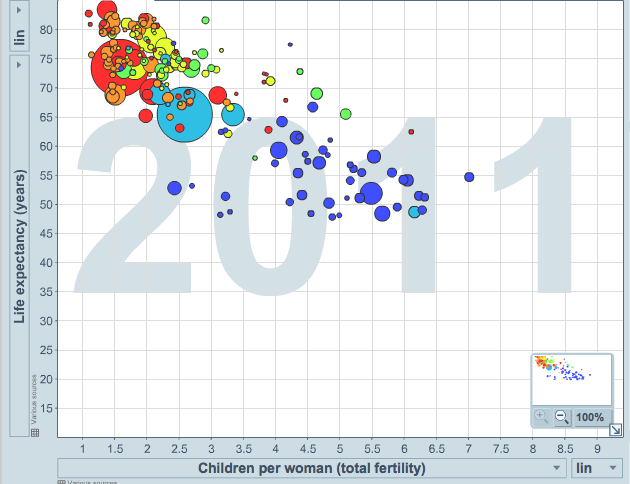
\includegraphics[width=\textwidth]{2-1_numerical_data/figures/life_exp_child}

\end{columns}

\ct{\webURL{http://www.gapminder.org/world}}

\end{frame}

%%%%%%%%%%%%%%%%%%%%%%%%%%%%%%%%%%%%

\subsection{Dot plots and the mean}

%%%%%%%%%%%%%%%%%%%%%%%%%%%%%%%%%%%%

\begin{frame}
\frametitle{Dot plots}

Useful for visualizing one numerical variable. Darker colors represent areas where there are more observations.

\begin{center}
%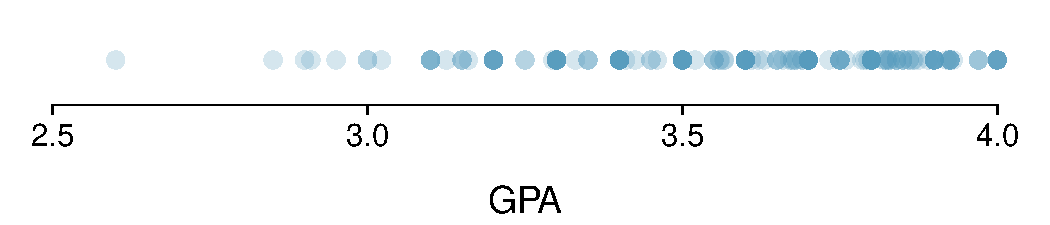
\includegraphics[width=\textwidth]{2-1_numerical_data/figures/gpa_dot_plot/gpa_dot_plot}
\end{center}

\dq{How would you describe the distribution of GPAs in this data set? Make sure to say something about the center, shape, and spread of the distribution.}

\end{frame}

%%%%%%%%%%%%%%%%%%%%%%%%%%%%%%%%%%%%


\begin{frame}
\frametitle{Dot plots \& mean}

\begin{center}
%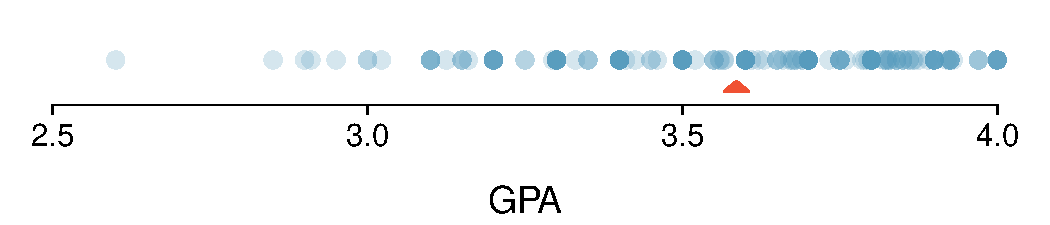
\includegraphics[width=\textwidth]{2-1_numerical_data/figures/gpa_dot_plot/gpa_dot_plot_mean}
\end{center}

\begin{itemize}

\item The \hl{mean}, also called the \hl{average} (marked with a triangle in the above plot), is one way to measure the center of a \hl{distribution} of data.

\item The mean GPA is 3.59.

\end{itemize} 

\end{frame}

%%%%%%%%%%%%%%%%%%%%%%%%%%%%%%%%%%%%

\begin{frame}
\frametitle{Mean}

\begin{itemize}

\item The \hl{sample mean}, denoted as \mathhl{\bar{x}}, can be calculated as

\[ \bar{x} = \frac{x_1 + x_2 + \cdots + x_n}{n}, \]

where $x_1, x_2, \cdots, x_n$ represent the \hl{n} observed values.

\item The \hl{population mean} is also computed the same way but is denoted as \mathhl{\mu}. It is often not possible to calculate $\mu$ since population data are rarely available.

\item The sample mean is a \hl{sample statistic}, and serves as a \hl{point estimate} of the population mean. This estimate may not be perfect, but if the sample is good (representative of the population), it is usually a pretty good estimate. 

\end{itemize}

\end{frame}

%%%%%%%%%%%%%%%%%%%%%%%%%%%%%%%%%%%%

\begin{frame}
\frametitle{Stacked dot plot}

Higher bars represent areas where there are more observations, makes it a little easier to judge the center and the shape of the distribution.

\begin{center}
%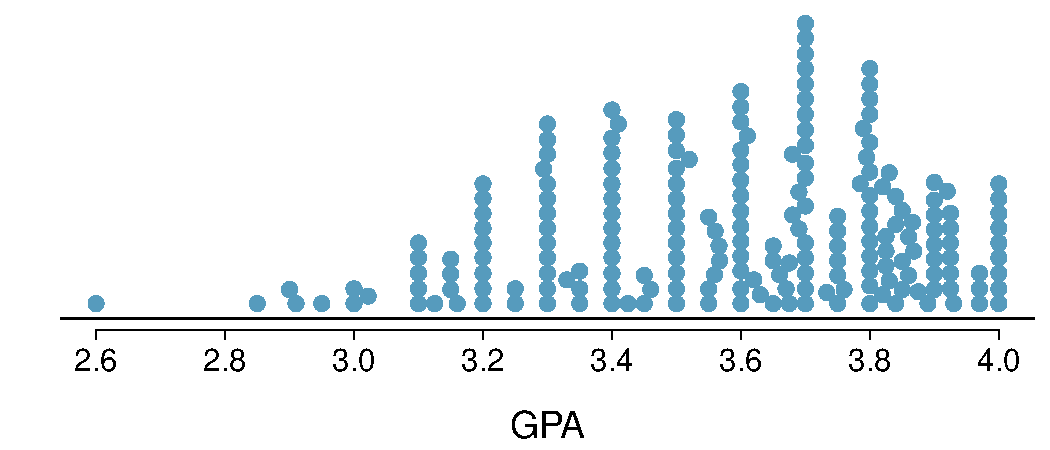
\includegraphics[width=\textwidth]{2-1_numerical_data/figures/gpa_dot_plot/gpa_dot_plot_stacked}
\end{center}

\end{frame}

%%%%%%%%%%%%%%%%%%%%%%%%%%%%%%%%%%%%

\subsection{Histograms and shape}

%%%%%%%%%%%%%%%%%%%%%%%%%%%%%%%%%%%%

\begin{frame}[fragile]
\frametitle{Histograms - Extracurricular hours}

\begin{itemize}

\item Histograms provide a view of the \hl{data density}. Higher bars represent where the data are relatively more common.

\item Histograms are especially convenient for describing the \hl{shape} of the data distribution.

\item The chosen \hl{bin width} can alter the story the histogram is telling.

\end{itemize}

\begin{center}
%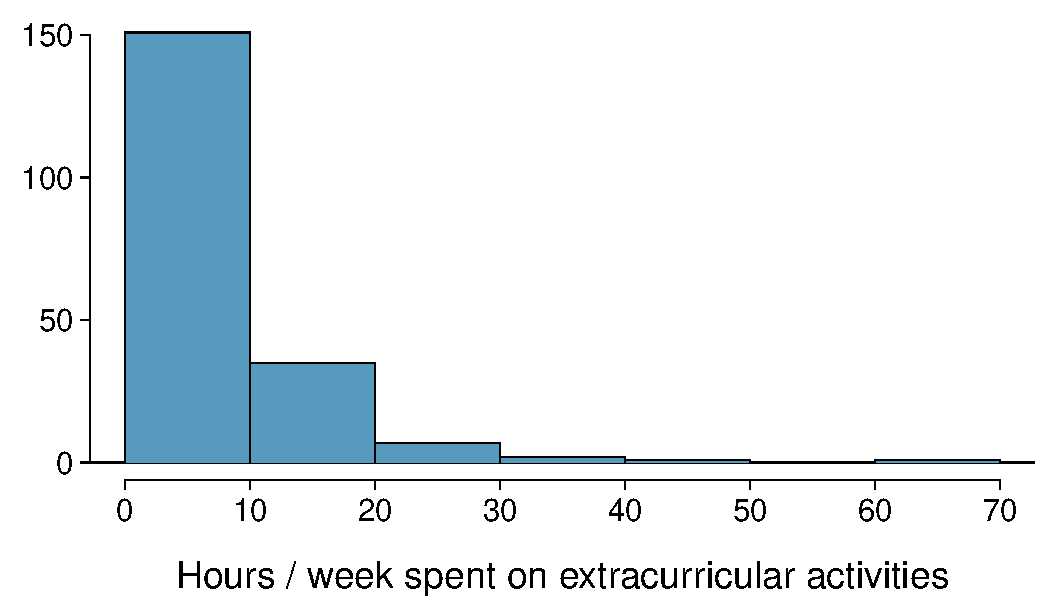
\includegraphics[width=0.75\textwidth]{2-1_numerical_data/figures/extracurr_hrs_hist/extracurr_hrs_hist}
\end{center}

\end{frame}

%%%%%%%%%%%%%%%%%%%%%%%%%%%%%%%%%%%%

\begin{frame}
\frametitle{Bin width}

\dq{Which one(s) of these histograms are useful? Which reveal too much about the data? Which hide too much?}

\begin{center}
%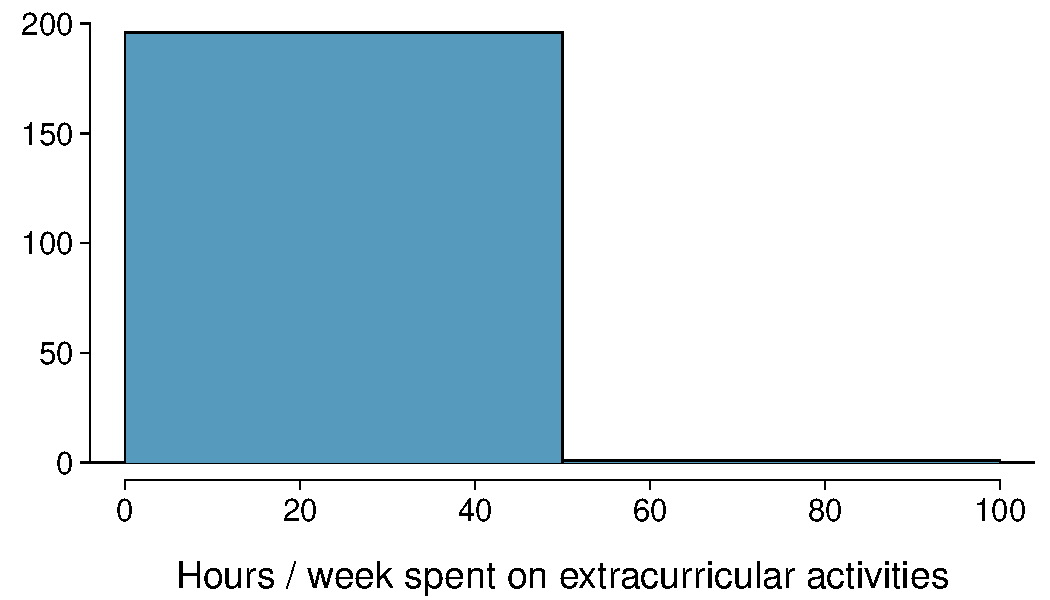
\includegraphics[width=0.45\textwidth]{2-1_numerical_data/figures/extracurr_hrs_hist/extracurr_hrs_hist2}
%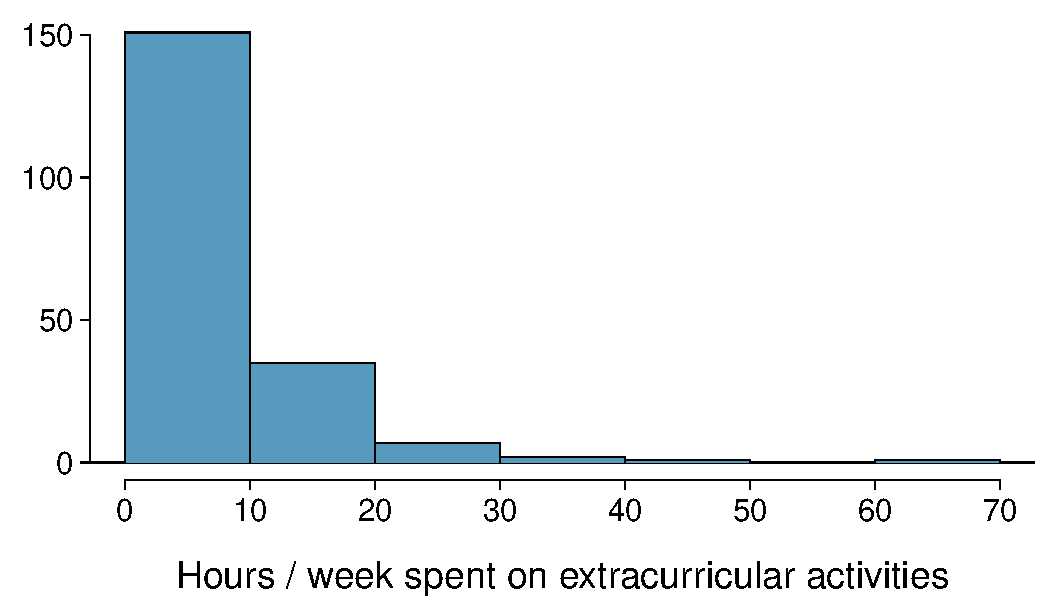
\includegraphics[width=0.45\textwidth]{2-1_numerical_data/figures/extracurr_hrs_hist/extracurr_hrs_hist} \\
%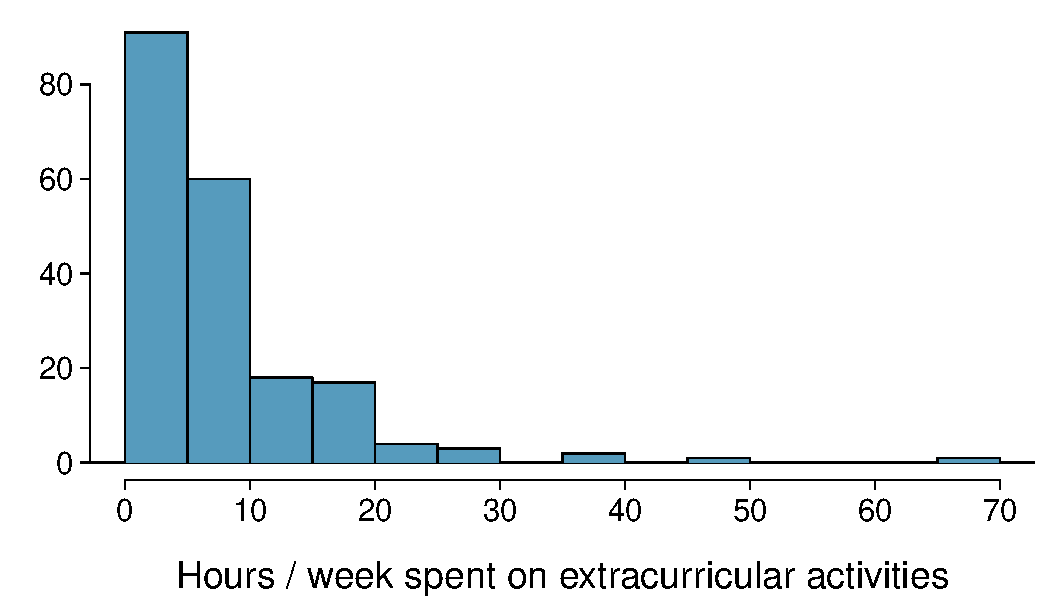
\includegraphics[width=0.45\textwidth]{2-1_numerical_data/figures/extracurr_hrs_hist/extracurr_hrs_hist20}
%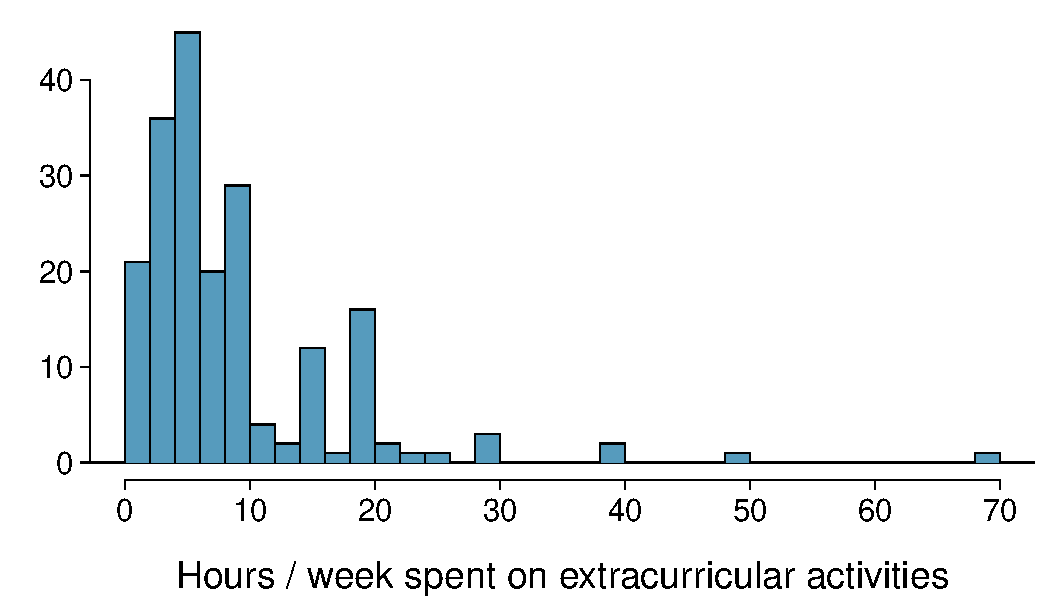
\includegraphics[width=0.45\textwidth]{2-1_numerical_data/figures/extracurr_hrs_hist/extracurr_hrs_hist30}
\end{center}

\end{frame}

%%%%%%%%%%%%%%%%%%%%%%%%%%%%%%%%%%%%

\begin{frame}
\frametitle{Shape of a distribution: modality}

Does the histogram have a single prominent peak (\hl{unimodal}), several prominent peaks (\hl{bimodal/multimodal}), or no apparent peaks (\hl{uniform})?

\begin{center}
%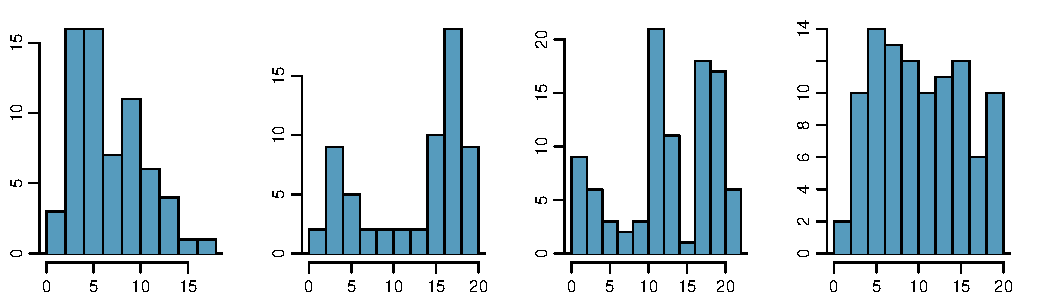
\includegraphics[width=0.75\textwidth]{2-1_numerical_data/figures/singleBiMultiModalUnifPlots/singleBiMultiModalUnifPlots}
\end{center}

\Note{In order to determine modality, step back and imagine a smooth curve over the histogram -- imagine that the bars are wooden blocks and you drop a limp spaghetti over them, the shape the spaghetti would take could be viewed as a smooth curve.}

\end{frame}

%%%%%%%%%%%%%%%%%%%%%%%%%%%%%%%%%%%%

\begin{frame}
\frametitle{Shape of a distribution: skewness}

Is the histogram \hl{right skewed}, \hl{left skewed}, or \hl{symmetric}?

\begin{center}
%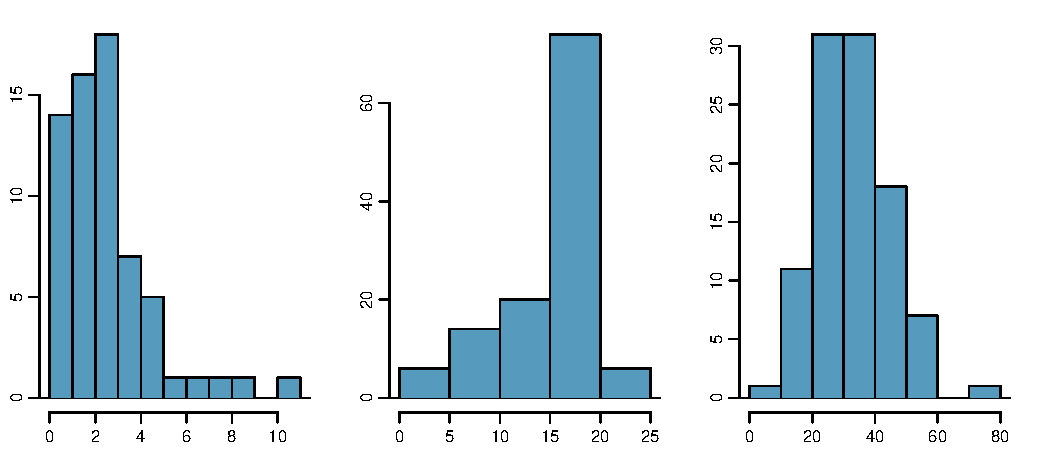
\includegraphics[width=0.8\textwidth]{2-1_numerical_data/figures/skewedSymPlots/skewedSymPlots}
\end{center}

\Note{Histograms are said to be skewed to the side of the long tail.}

\end{frame}

%%%%%%%%%%%%%%%%%%%%%%%%%%%%%%%%%%%%

\begin{frame}
\frametitle{Shape of a distribution: unusual observations}

Are there any unusual observations or potential \hl{outliers}?

\begin{center}
%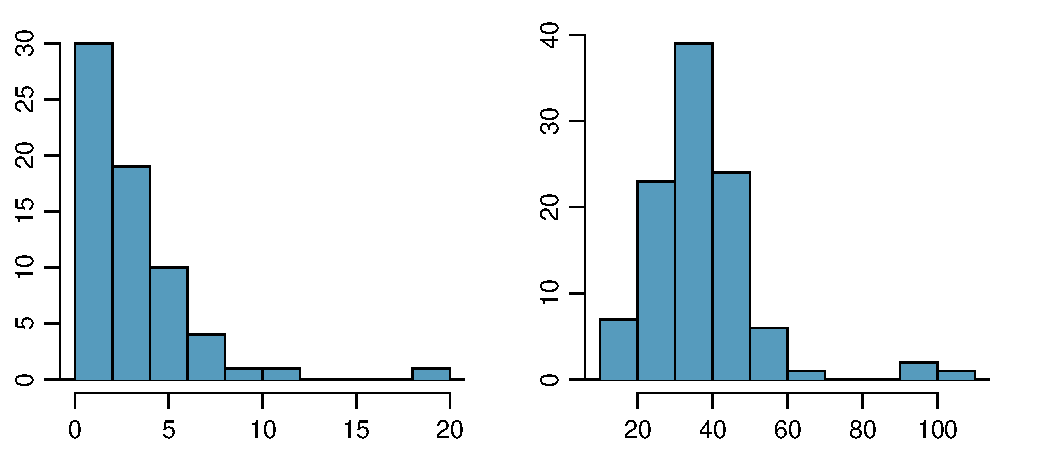
\includegraphics[width=0.8\textwidth]{2-1_numerical_data/figures/outlierPlots/outlierPlots}
\end{center}

\end{frame}

%%%%%%%%%%%%%%%%%%%%%%%%%%%%%%%%%%%%

\begin{frame}
\frametitle{Extracurricular activities}

\dq{How would you describe the shape of the distribution of hours per week students spend on extracurricular activities?}

\begin{center}
%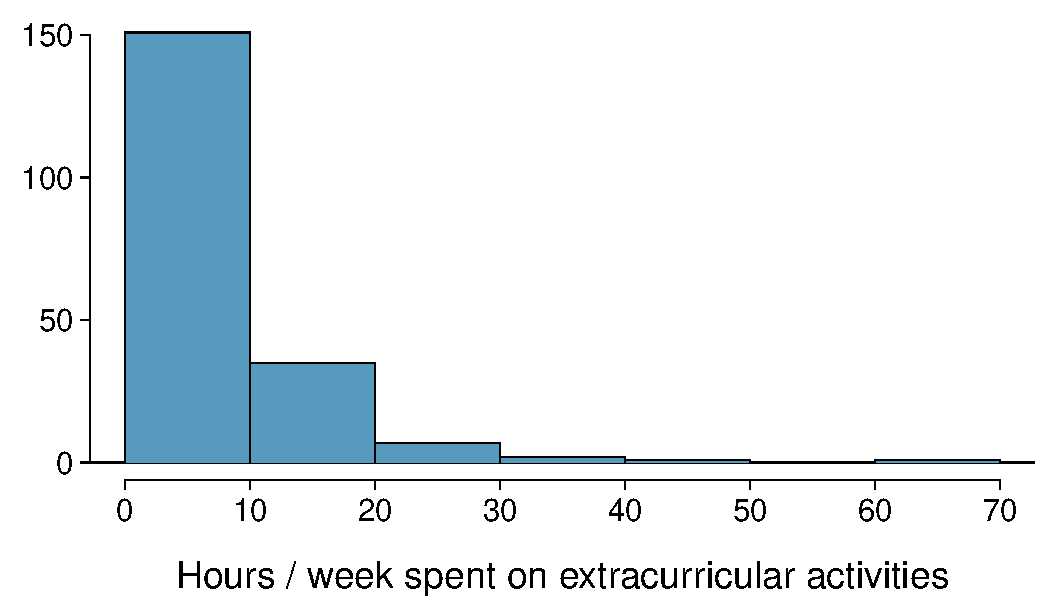
\includegraphics[width=0.75\textwidth]{2-1_numerical_data/figures/extracurr_hrs_hist/extracurr_hrs_hist}
\end{center}

\soln{\pause{Unimodal and right skewed, with a potentially unusual observation at 60 hours/week.}}

\end{frame}

%%%%%%%%%%%%%%%%%%%%%%%%%%%%%%%%%%%%

\begin{frame}
\frametitle{Commonly observed shapes of distributions}

\begin{itemize}

\item modality \\
$\:$ \\
\pause

\begin{columns}[c]
\column{0.25\textwidth}
unimodal \\
%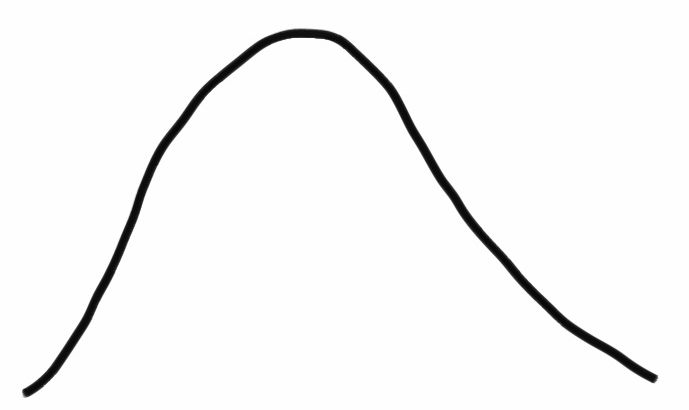
\includegraphics[width=\textwidth]{2-1_numerical_data/figures/shape_sketches/unimodal} 
\pause
\column{0.25\textwidth}
bimodal \\
%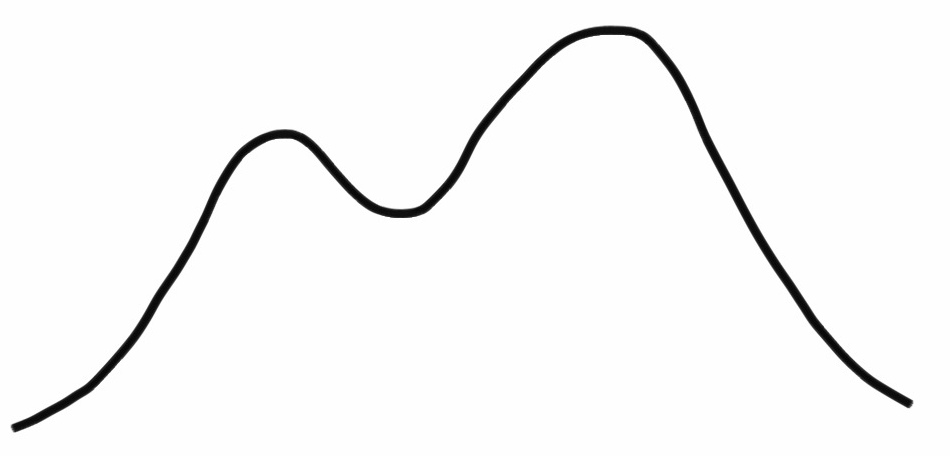
\includegraphics[width=\textwidth]{2-1_numerical_data/figures/shape_sketches/bimodal} 
\pause
\column{0.25\textwidth}
multimodal \\
%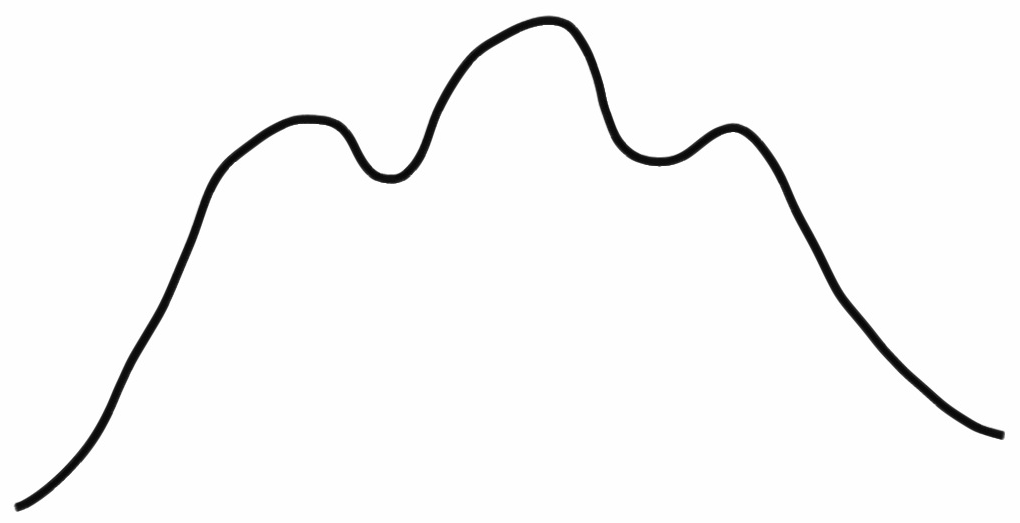
\includegraphics[width=\textwidth]{2-1_numerical_data/figures/shape_sketches/multimodal} 
\pause
\column{0.25\textwidth}
uniform
%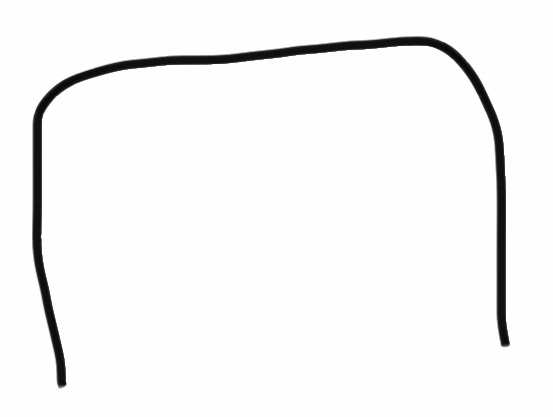
\includegraphics[width=\textwidth]{2-1_numerical_data/figures/shape_sketches/uniform} 
\end{columns}

\pause

$\:$ \\

\item skewness \\
$\:$ \\
\pause

\begin{columns}[c]
\column{0.25\textwidth}
right skew \\
%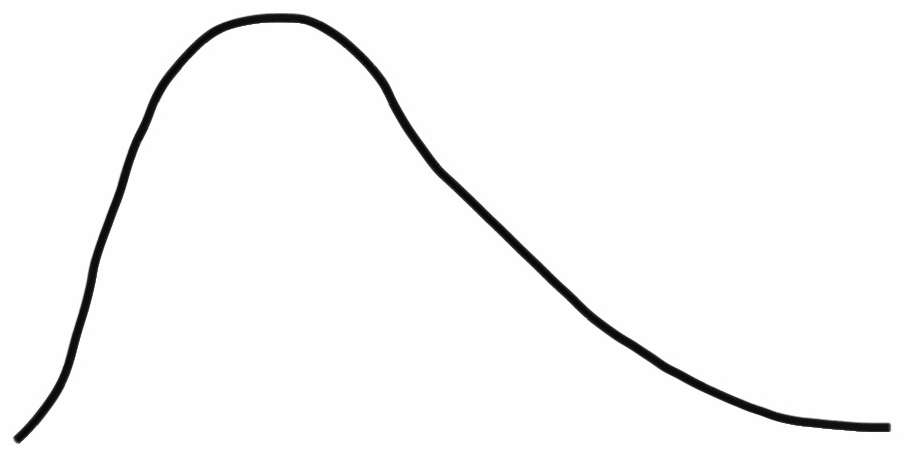
\includegraphics[width=\textwidth]{2-1_numerical_data/figures/shape_sketches/right_skew} 
\pause
\column{0.25\textwidth}
left skew \\
%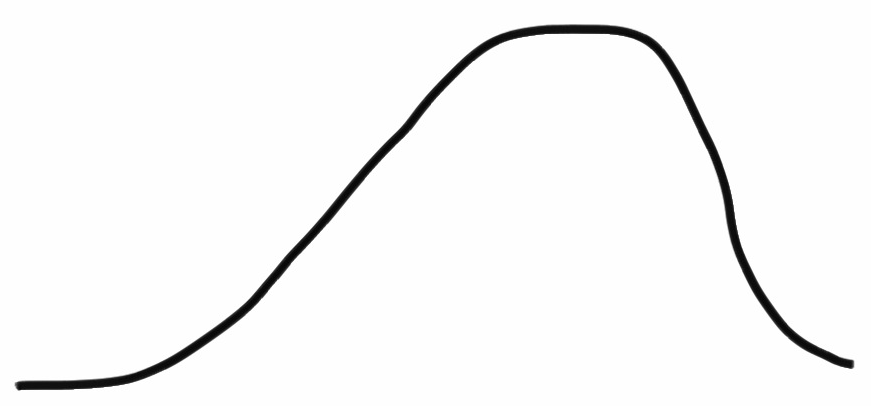
\includegraphics[width=\textwidth]{2-1_numerical_data/figures/shape_sketches/left_skew} 
\pause
\column{0.25\textwidth}
symmetric \\
%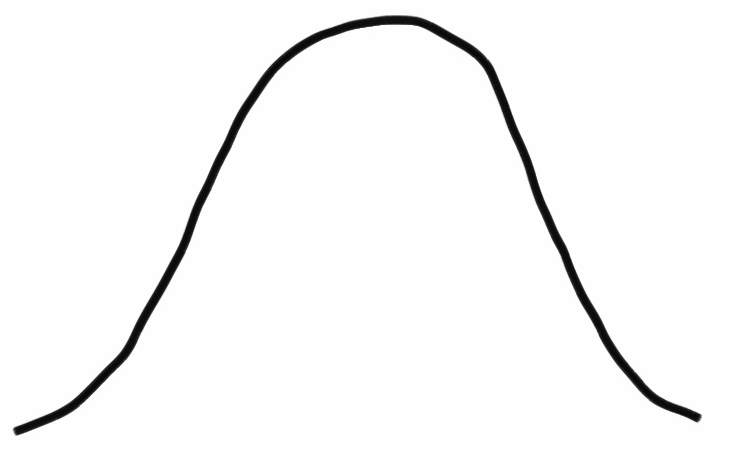
\includegraphics[width=\textwidth]{2-1_numerical_data/figures/shape_sketches/symmetric} 
\end{columns}

\end{itemize}

\end{frame}

%%%%%%%%%%%%%%%%%%%%%%%%%%%%%%%%%%%

\begin{frame}
\frametitle{Practice}

\pq{Which of these variables do you expect to be uniformly distributed?}

\begin{enumerate}[(a)]
\item weights of adult females
\item salaries of a random sample of people from North Carolina
\item house prices
\solnMult{birthdays of classmates (day of the month)}
\end{enumerate}

\end{frame}

%%%%%%%%%%%%%%%%%%%%%%%%%%%%%%%%%%%

\begin{frame}
\frametitle{Application activity: Shapes of distributions}

\app{Sketch the expected distributions of the following variables:
\begin{itemize}
\item number of piercings
\item scores on an exam
\item IQ scores
\end{itemize}
Come up with a concise way (1-2 sentences) to teach someone how to determine the expected distribution of any variable.
}

\end{frame}

%%%%%%%%%%%%%%%%%%%%%%%%%%%%%%%%%%%

\begin{frame}
\frametitle{Are you typical?}

\begin{center}
%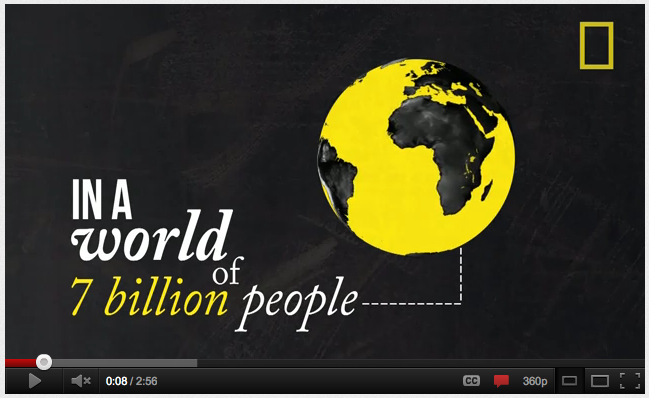
\includegraphics[width=0.75\textwidth]{2-1_numerical_data/figures/typical}
\end{center}

\begin{center}
\footnotesize{\webURL{http://www.youtube.com/watch?v=4B2xOvKFFz4}}
\end{center}

\pause

\dq{How useful are centers alone for conveying the true characteristics of a distribution?}

\end{frame}

%%%%%%%%%%%%%%%%%%%%%%%%%%%%%%%%%%%%

\subsection{Variance and standard deviation}

%%%%%%%%%%%%%%%%%%%%%%%%%%%%%%%%%%%

\begin{frame}
\frametitle{Variance}

\hl{Variance} is roughly the average squared deviation from the mean.

\formula{
\[ s^2 = \frac{\sum_{i = 1}^n (x_i - \bar{x})^2}{n - 1} \]
}

\pause

\twocol{0.5}{0.5}
{
\begin{itemize}

\item The sample mean is $\bar{x} = 6.71$, and the sample size is $n = 217$.

\onslide<3->{\item The variance of amount of sleep students get per night can be calculated as:}
\end{itemize}
}
{
\onslide<2->{
\begin{center}
%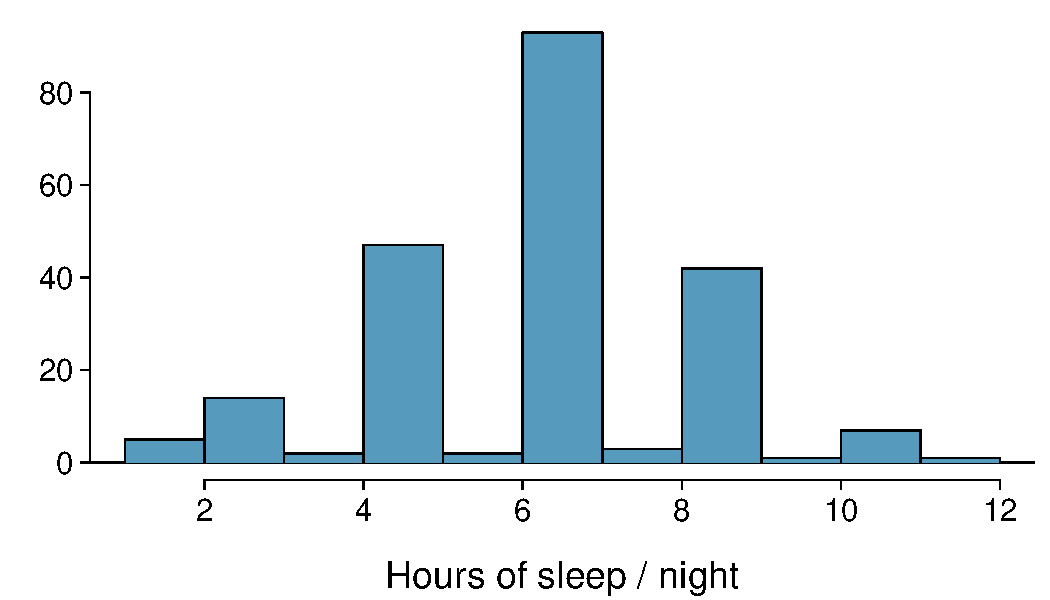
\includegraphics[width=\textwidth]{2-1_numerical_data/figures/sleep_hist/sleep_hist}
\end{center}
}
}
$\:$
\onslide<3->{
\[ s^2 = \frac{(5 - 6.71)^2 + (9 - 6.71)^2 + \cdots + (7 - 6.71)^2}{217 - 1} = 4.11~hours^2 \]
}



\end{frame}

%%%%%%%%%%%%%%%%%%%%%%%%%%%%%%%%%%%

\begin{frame}
\frametitle{Variance (cont.)}

\dq{Why do we use the squared deviation in the calculation of variance?}

\soln{\pause
\begin{itemize}
\item To get rid of negatives so that observations equally distant from the mean are weighed equally.
\item To weigh larger deviations more heavily.
\end{itemize}
}

\end{frame}

%%%%%%%%%%%%%%%%%%%%%%%%%%%%%%%%%%

\begin{frame}
\frametitle{Standard deviation}

The \hl{standard deviation} is the square root of the variance, and has the same units as the data

\formula{
\[ s = \sqrt{s^2} \]
}

\pause

\twocol{0.5}{0.5}
{
\begin{itemize}

\item The standard deviation of amount of sleep students get per night can be calculated as:
\[ s = \sqrt{4.11} = 2.03~hours\]

\onslide<3->{\item We can see that all of the data are within 3 standard deviations of the mean.}
\end{itemize}
}
{
\onslide<2->{
\begin{center}
%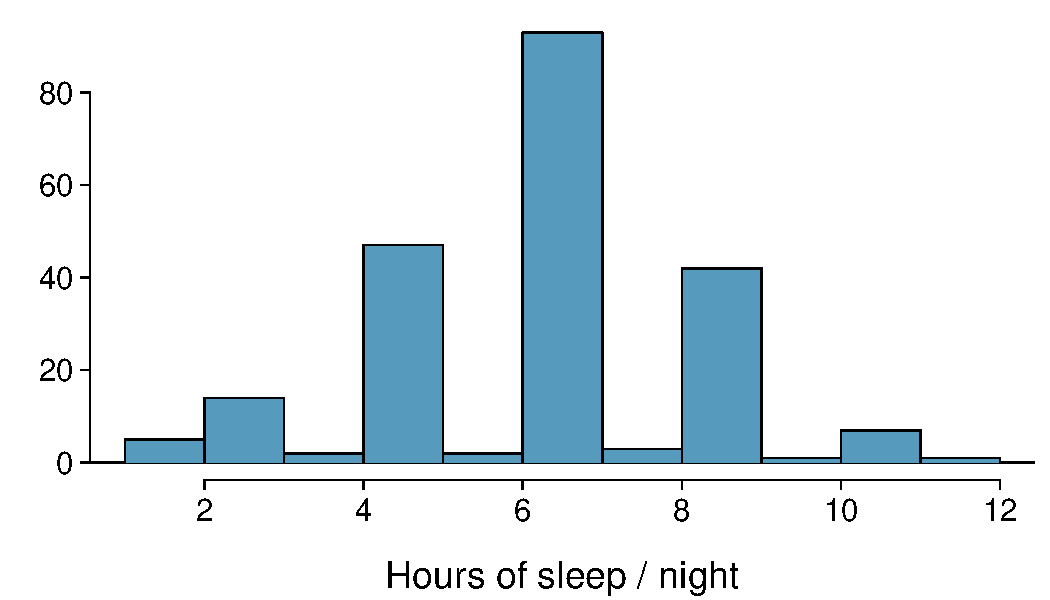
\includegraphics[width=\textwidth]{2-1_numerical_data/figures/sleep_hist/sleep_hist}
\end{center}
}
}

\end{frame}

%%%%%%%%%%%%%%%%%%%%%%%%%%%%%%%%%%%%

\subsection{Box plots, quartiles, and the median}

%%%%%%%%%%%%%%%%%%%%%%%%%%%%%%%%%%%%

\begin{frame}
\frametitle{Median}

\begin{itemize}

\item The \hl{median} is the value that splits the data in half when ordered in ascending order.

\[ 0,1,\orange{2},3,4 \]

\item If there are an even number of observations, then the median is the average of the two values in the middle.

\[ 0,1,\underline{2,3},4,5 \rightarrow \frac{2 + 3}{2} = \orange{2.5} \]

\item Since the median is the midpoint of the data, 50\% of the values are below it. Hence, it is also the \hl{$50^{th}$ percentile}.

\end{itemize}

\end{frame}

%%%%%%%%%%%%%%%%%%%%%%%%%%%%%%%%%%%%

\begin{frame}[fragile]
\frametitle{Q1, Q3, and IQR}

\begin{itemize}

\item The $25^{th}$ percentile is also called the first quartile, \hl{Q1}.

\item The $50^{th}$ percentile is also called the median.

\item The $75^{th}$ percentile is also called the third quartile, \hl{Q3}.

\item Between Q1 and Q3 is the middle 50\% of the data. The range these data span is called the \hl{interquartile range}, or the \hl{IQR}.
\formula{\[ IQR = Q3 - Q1 \]}
\end{itemize}

\end{frame}

%%%%%%%%%%%%%%%%%%%%%%%%%%%%%%%%%%%%

\begin{frame}
\frametitle{Box plot}

The box in a \hl{box plot} represents the middle 50\% of the data, and the thick line in the box is the median.

\begin{center}
%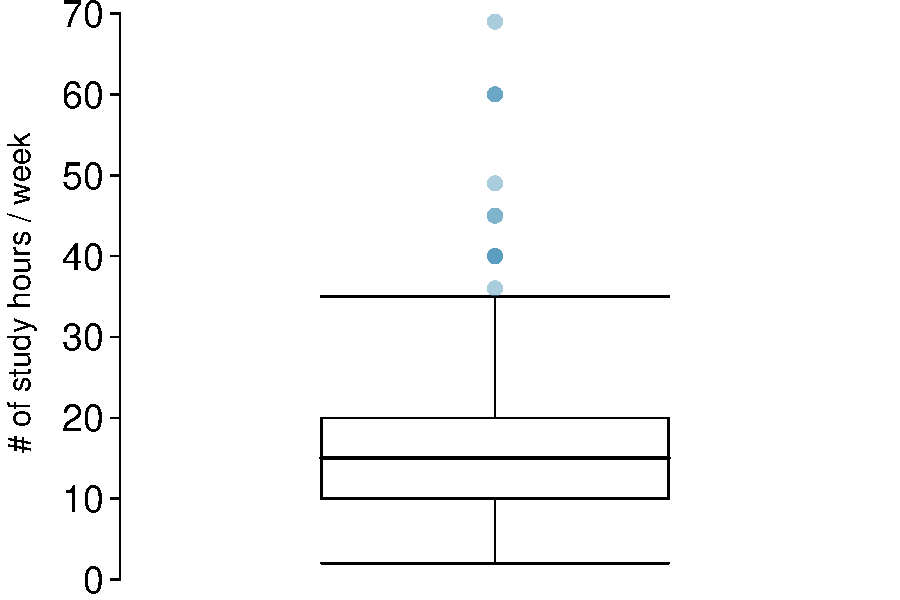
\includegraphics[width=0.7\textwidth]{2-1_numerical_data/figures/study_hours/study_hours_box}
\end{center}

\end{frame}

%%%%%%%%%%%%%%%%%%%%%%%%%%%%%%%%%%%%

\begin{frame}
\frametitle{Anatomy of a box plot}

\begin{center}
%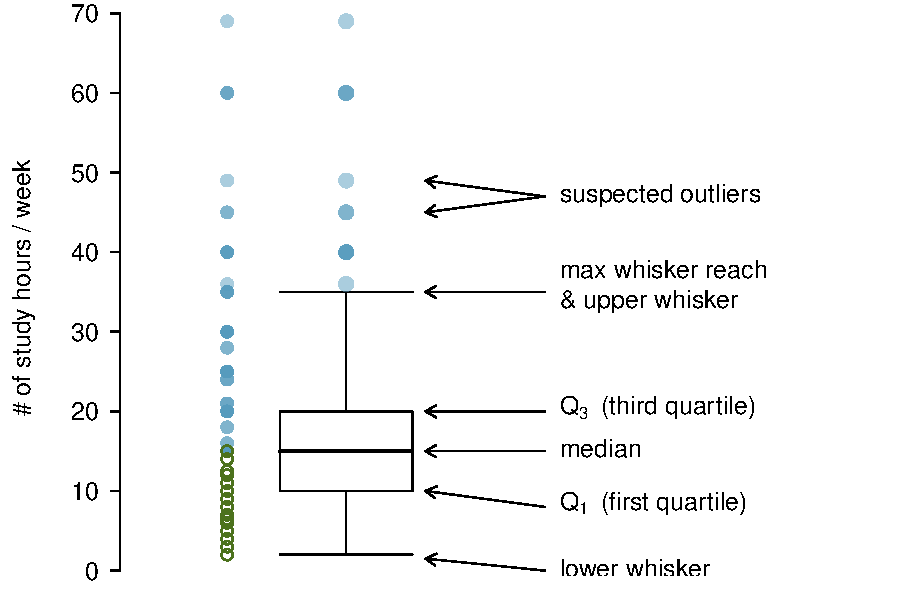
\includegraphics[width=0.95\textwidth]{2-1_numerical_data/figures/study_hours/study_hours_box_layout}
\end{center}

\end{frame}

%%%%%%%%%%%%%%%%%%%%%%%%%%%%%%%%%%%%

\begin{frame}[fragile]
\frametitle{Whiskers and outliers}

\begin{itemize}

\item \hl{Whiskers} of a box plot can extend up to $1.5 \times IQR$ away from the quartiles.
\formula{
\vspace{-0.5cm}
\begin{align*} 
\text{max~upper~whisker~reach} &= Q3 + 1.5 \times IQR \\
\text{max~lower~whisker~reach} &= Q1 - 1.5 \times IQR
\end{align*}
}
\pause
\vspace{-0.5cm}
{\small
\begin{align*}
\text{IQR}&: 20 - 10 = 10 \\
\text{max~upper~whisker~reach}&= 20 + 1.5 \times 10 = 35 \\
\text{max~lower~whisker~reach}&= 10 - 1.5 \times 10 = -5
\end{align*}
}

\pause
\vspace{-0.25cm}
\item A potential \hl{outlier} is defined as an observation beyond the maximum reach of the whiskers. It is an observation that appears extreme relative to the rest of the data.

\end{itemize}

\end{frame}

%%%%%%%%%%%%%%%%%%%%%%%%%%%%%%%%%%%%

\begin{frame}
\frametitle{Outliers (cont.)}

\dq{Why is it important to look for outliers?}

\soln{
\onslide<2->{
\begin{itemize}
\item Identify extreme skew in the distribution.
\item Identify data collection and entry errors.
\item Provide insight into interesting features of the data.
\end{itemize}
}
}

\end{frame}

%%%%%%%%%%%%%%%%%%%%%%%%%%%%%%%%%%%%

\subsection{Robust statistics}

%%%%%%%%%%%%%%%%%%%%%%%%%%%%%%%%%%%%

\begin{frame}
\frametitle{Extreme observations}

\dq{How would sample statistics such as mean, median, SD, and IQR of household income be affected if the largest value was replaced with \$10 million? What if the smallest value was replaced with \$10 million?}

\begin{center}
%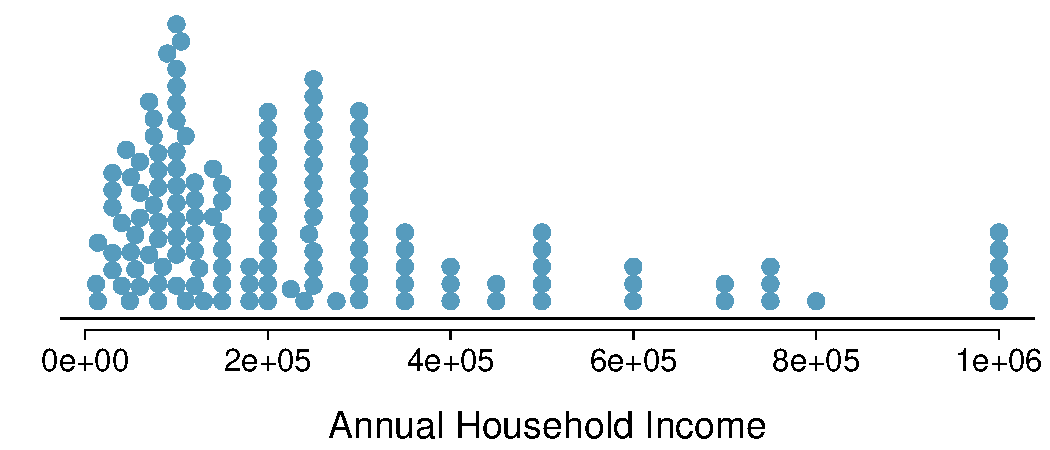
\includegraphics[width=\textwidth]{2-1_numerical_data/figures/house_income/house_income_dot_stacked}
\end{center}

\end{frame}

%%%%%%%%%%%%%%%%%%%%%%%%%%%%%%%%%%%%

\begin{frame}
\frametitle{Robust statistics}

\begin{center}
%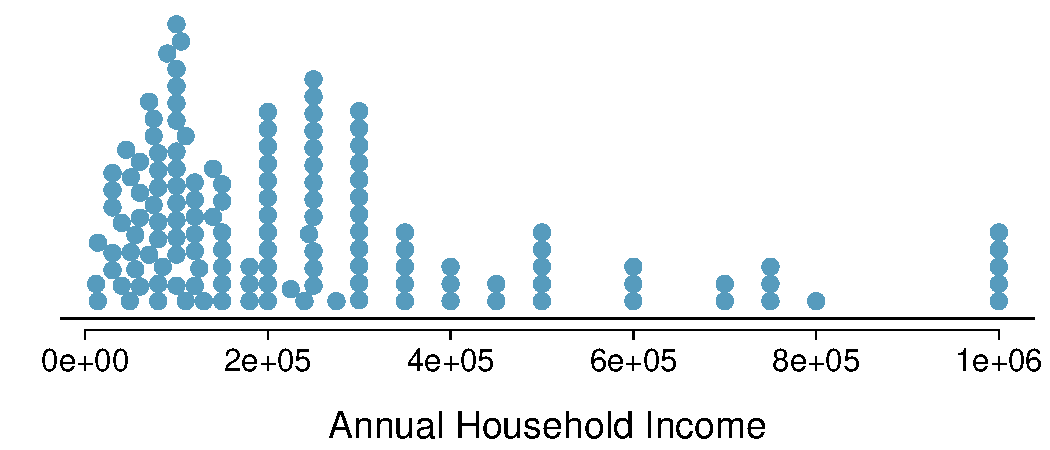
\includegraphics[width=\textwidth]{2-1_numerical_data/figures/house_income/house_income_dot_stacked}
\end{center}

{\small
\begin{center}
\begin{tabular}{l c cc c cc}
  \hline
& \hspace{0mm} & \multicolumn{2}{c}{\bf robust} & \hspace{2mm} & \multicolumn{2}{c}{\bf not robust} \\
scenario && median & IQR && $\bar{x}$ & $s$ \\ 
  \hline
original data && 190K & 200K && 245K & 226K \\ 
move largest to \$10 million && 190K & 200K && 309K & 853K \\ 
move smallest to \$10 million && 200K & 200K && 316K & 854K \\ 
   \hline
\end{tabular}
\end{center}
}

\end{frame}

%%%%%%%%%%%%%%%%%%%%%%%%%%%%%%%%%%%%

\begin{frame}
\frametitle{Robust statistics}

Median and IQR are more robust to skewness and outliers than mean and SD. Therefore,

\begin{itemize}
\item for skewed distributions it is often more helpful to use median and IQR to describe the center and spread
\item for symmetric distributions it is often more helpful to use the mean and SD to describe the center and spread
\end{itemize}

$\:$ \\

\pause

\dq{If you would like to estimate the typical household income for a student, would you be more interested in the mean or median income?}

\soln{\pause{Median}}

\end{frame}

%%%%%%%%%%%%%%%%%%%%%%%%%%%%%%%%%%%%

\begin{frame}
\frametitle{Mean vs. median}

\begin{itemize}

\item If the distribution is symmetric, center is often defined as the mean: mean $\approx$ median

\begin{center}
%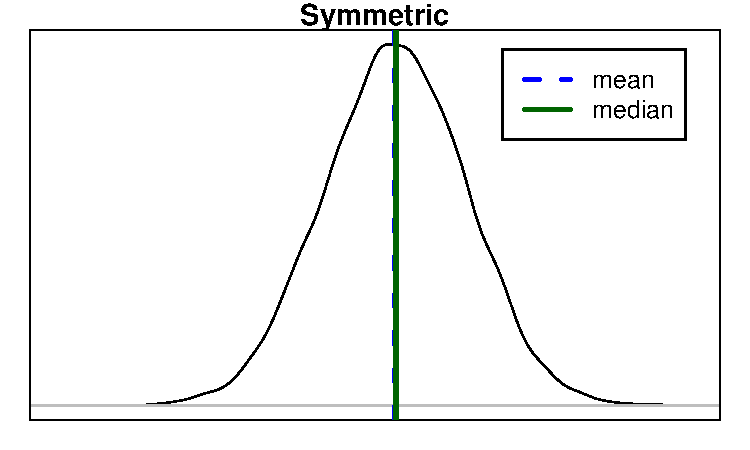
\includegraphics[width=0.33\textwidth]{2-1_numerical_data/figures/mean_med/sym}
\end{center}

\item If the distribution is skewed or has extreme outliers, center is often defined as the median
\begin{itemize}
\item Right-skewed: mean $>$ median
\item Left-skewed: mean $<$ median \\
\end{itemize}

\end{itemize}

\begin{center}
%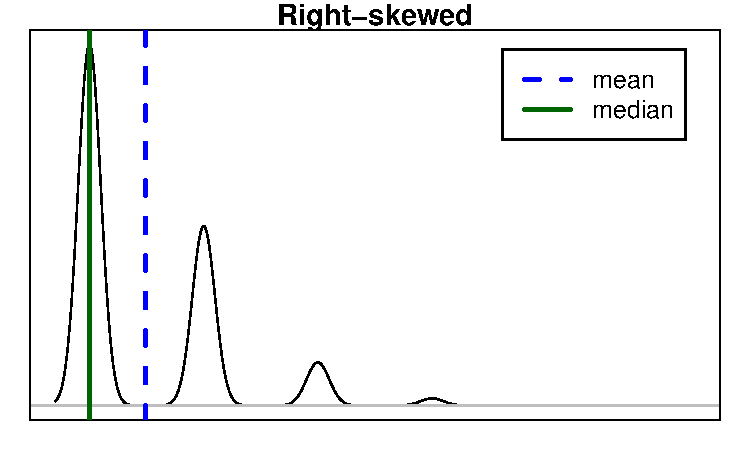
\includegraphics[width=0.33\textwidth]{2-1_numerical_data/figures/mean_med/rs}
%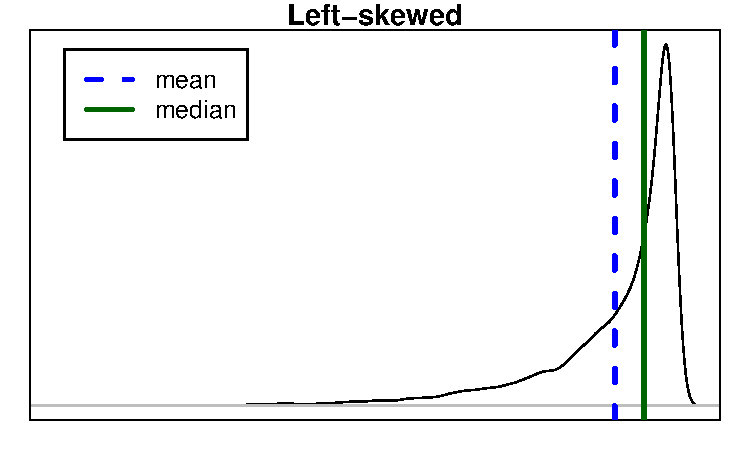
\includegraphics[width=0.33\textwidth]{2-1_numerical_data/figures/mean_med/ls}\\
\end{center}

\end{frame}

%%%%%%%%%%%%%%%%%%%%%%%%%%%%%%%%%%%%%

\begin{frame}
\frametitle{Practice}

\pq{{\small Which is most likely true for the distribution of percentage of time actually spent taking notes in class versus on Facebook, Twitter, etc.?}}

\vspace{-0.5cm}

\begin{columns}
\column{0.7\textwidth}
\begin{center}
%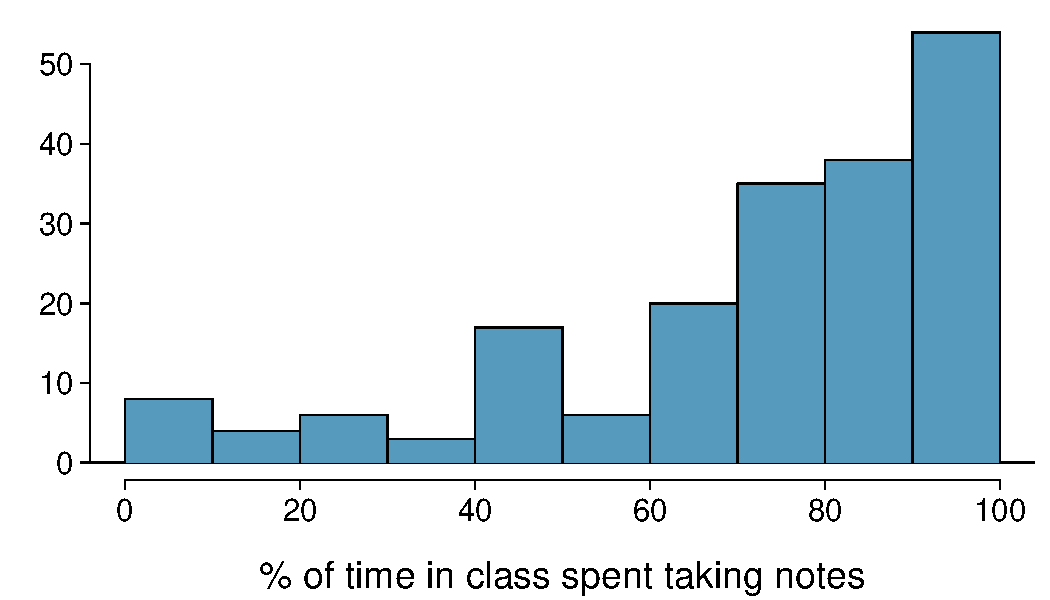
\includegraphics[width=0.9\textwidth]{2-1_numerical_data/figures/notes_perc/notes_perc_hist}
\end{center}
\column{0.3\textwidth}
$\:$ \\
$\:$ \\
\soln{\only<2>{\orange{median: 80\% \\ mean: 76\%}}}
\end{columns}

{\small
\begin{multicols}{2}
\begin{enumerate}[(a)]
\item mean$>$ median
\solnMult{mean $<$ median}
\item mean $\approx$ median
\item impossible to tell
\end{enumerate}
\end{multicols}
}

\end{frame}

%%%%%%%%%%%%%%%%%%%%%%%%%%%%%%%%%%%%%

\subsection{Transforming data}

%%%%%%%%%%%%%%%%%%%%%%%%%%%%%%%%%%%%

\begin{frame}
\frametitle{Extremely skewed data}

When data are extremely skewed, transforming them might make modeling easier. A common transformation is the \hl{log transformation}.

$\:$ \\
\pause
The histograms on the left shows the distribution of number of basketball games attended by students. The histogram on the right shows the distribution of log of number of games attended.

\begin{center}
%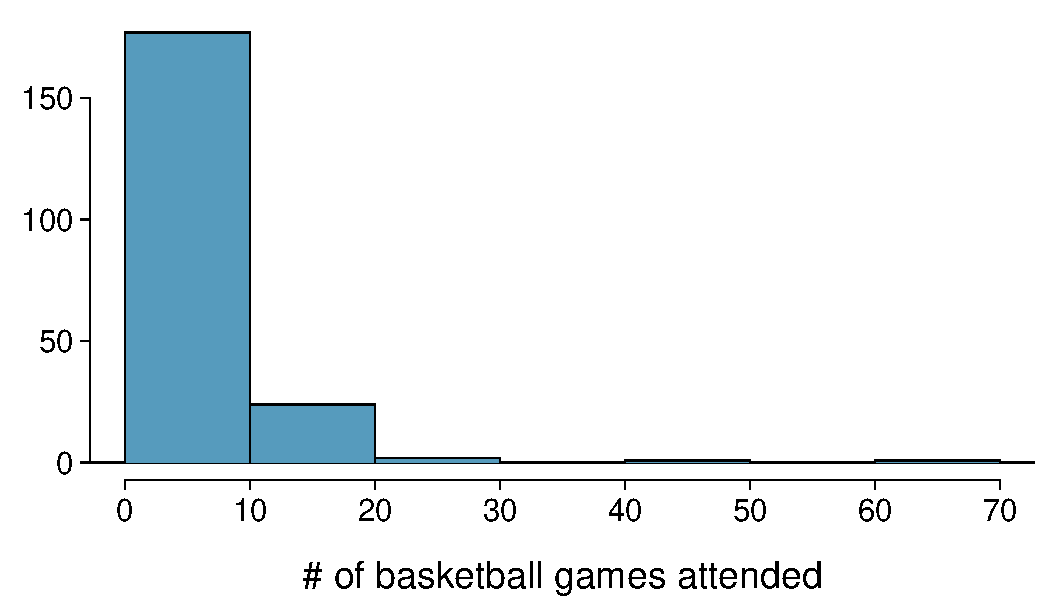
\includegraphics[width=0.5\textwidth]{2-1_numerical_data/figures/basket_games/basket_games_hist}
%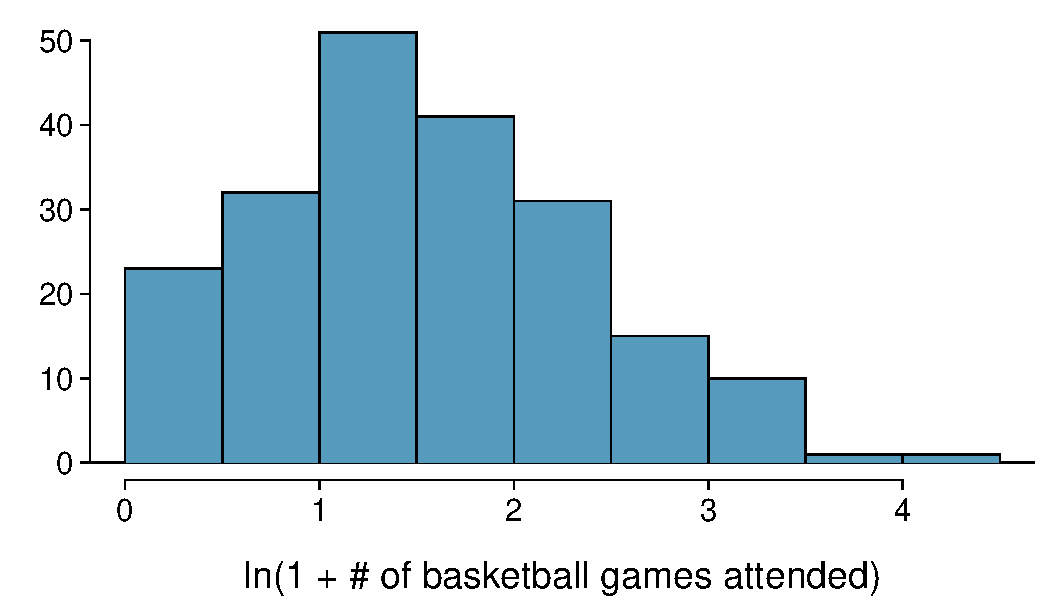
\includegraphics[width=0.5\textwidth]{2-1_numerical_data/figures/basket_games/basket_games_hist_log}
\end{center}

\end{frame}

%%%%%%%%%%%%%%%%%%%%%%%%%%%%%%%%%%%%

\begin{frame}
\frametitle{Pros and cons of transformations}

\begin{itemize}

\item Skewed data are easier to model with when they are transformed because outliers tend to become far less prominent after an appropriate transformation. \\
$\:$ \\
\renewcommand{\arraystretch}{1.5}
\begin{tabular}{l r r r r }
\# of games		&  70 	& 50 		& 25 		 		& $\cdots$ \\
log(\# of games)	& 4.25	& 3.91 	& 3.22 	 	& $\cdots$
\end{tabular}

$\:$ \\

\item However, results of an analysis in log units of the measured variable might be difficult to interpret.

\end{itemize}

\pause

\dq{What other variables would you expect to be extremely skewed?}

\soln{\pause{Salary, housing prices, etc.}}

\end{frame}

%%%%%%%%%%%%%%%%%%%%%%%%%%%%%%%%%%%%

\subsection{Mapping data}

%%%%%%%%%%%%%%%%%%%%%%%%%%%%%%%%%%%%

\begin{frame}
\frametitle{Intensity maps}

\dq{What patterns are apparent in the change in population between 2000 and 2010?}

\begin{center}
%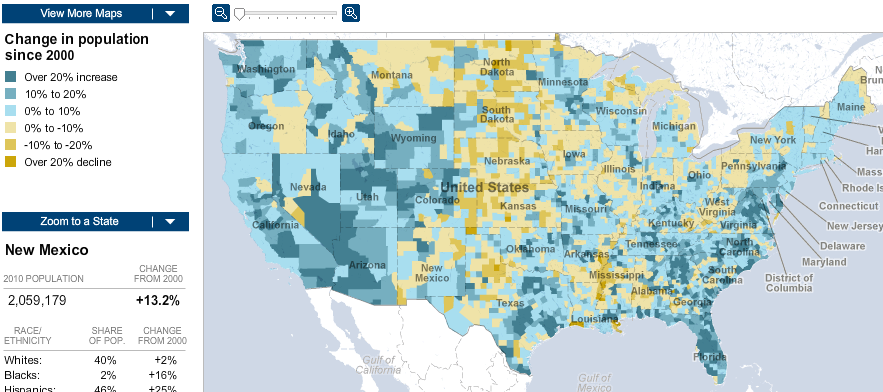
\includegraphics[width=0.95\textwidth]{2-1_numerical_data/figures/change_in_pop_intensity}
\end{center}

\ct{\webURL{http://projects.nytimes.com/census/2010/map}}

\end{frame}


%%%%%%%%%%%%%%%%%%%%%%%%%%%%%%%%%%%%

%%%%%%%%%%%%%%%%%%%%%%%%%%%%%%%%%%%%

\section{Considering categorical data}

%%%%%%%%%%%%%%%%%%%%%%%%%%%%%%%%%%%%

\subsection{Contingency tables and bar plots}

%%%%%%%%%%%%%%%%%%%%%%%%%%%%%%%%%%%%

\begin{frame}
\frametitle{Contingency tables}

A table that summarizes data for two categorical variables is called a \hl{contingency table}.

$\:$ \\
\pause
The contingency table below shows the distribution of survival and ages of passengers on the Titanic.

\begin{center}
\begin{tabular}{l l cc r}
					               & 			 & \multicolumn{2}{c}{{Survival}} \\
  \cline{3-4}
					               &			 & Died	 & Survived	& Total \\ 
  \cline{2-5}
\multirow{2}{*}{{Age}}& Adult & 1438  & 654 	  	& 2092 \\ 
  					             & Child & 52 	 & 57	 	    & 109\\ 
  \cline{2-5}
  					             & Total & 1490  & 711	    &  2201 \\
  \cline{2-5}
\end{tabular}
\end{center}
\end{frame}

%%%%%%%%%%%%%%%%%%%%%%%%%%%%%%%%%%%%

\begin{frame}
\frametitle{Bar plots}

A \hl{bar plot} is a common way to display a single categorical variable. A bar plot where proportions instead of frequencies are shown is called a \hl{relative frequency bar plot}.

\begin{center}
%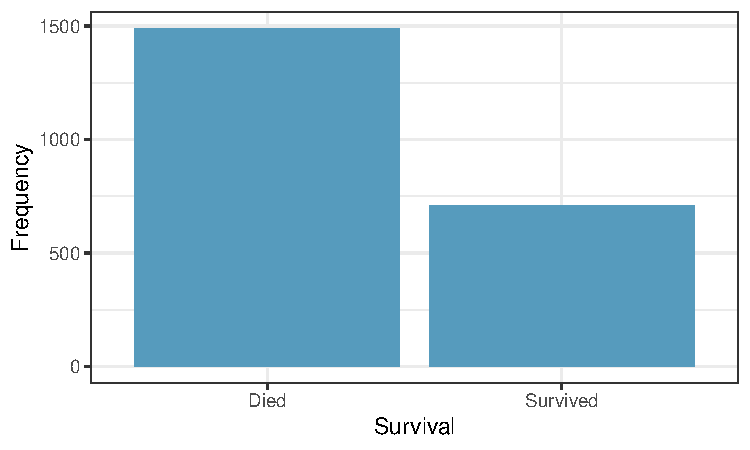
\includegraphics[width=0.45\textwidth]{2-2_categorical_data/figures/titanic_age_survival/titanic_bar}
%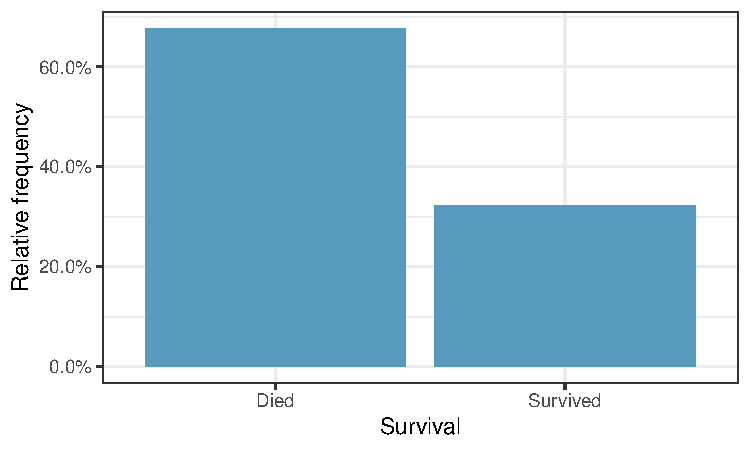
\includegraphics[width=0.45\textwidth]{2-2_categorical_data/figures/titanic_age_survival/titanic_rel_bar}
\end{center}

\pause

\dq{How are bar plots different than histograms?}

\soln{\pause{{\tiny Bar plots are used for displaying distributions of categorical variables,  histograms are used for numerical variables. The x-axis in a histogram is a number line,  hence the order of the bars cannot be changed. In a bar plot, the categories can be listed in any order (though some orderings make more sense than others, especially for ordinal variables.)}}}

\end{frame}

%%%%%%%%%%%%%%%%%%%%%%%%%%%%%%%%%%%%

\subsection{Row and column proportions}

%%%%%%%%%%%%%%%%%%%%%%%%%%%%%%%%%%%%

\begin{frame}
\frametitle{Choosing the appropriate proportion}

\dq{Does there appear to be a relationship between age and survival for passengers on the Titanic?}

\begin{center}
\begin{tabular}{l l cc r}
					               & 			 & \multicolumn{2}{c}{{Survival}} \\
  \cline{3-4}
					               &			 & Died	 & Survived	& Total \\ 
  \cline{2-5}
\multirow{2}{*}{{Age}}& Adult & 1438  & 654 	  	& 2092 \\ 
  					             & Child & 52 	 & 57	 	    & 109\\ 
  \cline{2-5}
  					             & Total & 1490  & 711	    &  2201 \\
  \cline{2-5}
\end{tabular}
\end{center}

\pause

To answer this question we examine the row proportions: 

\pause

\begin{itemize}

\item \% Adults who survived: 654 / 2092 $\approx 0.31$ \\

\pause

\item \% Children who survived: 57 / 109 $\approx 0.52$ \\

\end{itemize}

\end{frame}

%%%%%%%%%%%%%%%%%%%%%%%%%%%%%%%%%%%%

\subsection{Using a bar plot with two variables}

%%%%%%%%%%%%%%%%%%%%%%%%%%%%%%%%%%%%

\begin{frame}
\frametitle{Bar plots with two variables}

\begin{itemize}

\item \hl{Stacked bar plot:} Graphical display of contingency table information,
for counts.

\item \hl{Side-by-side bar plot:} Displays the same information by placing bars 
next to, instead of on top of, each other.

\item \hl{Standardized stacked bar plot}: Graphical display of contingency table 
information, for proportions.

\end{itemize}

\end{frame}

%%%%%%%%%%%%%%%%%%%%%%%%%%%%%%%%%%%%

\begin{frame}

\dq{What are the differences between the three visualizations shown below?}

\begin{center}
%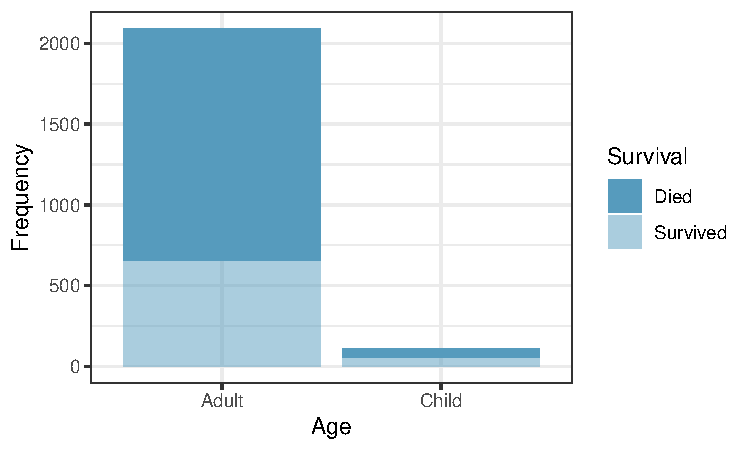
\includegraphics[width=0.5\textwidth]{2-2_categorical_data/figures/titanic_age_survival/titanic_seg_bar}
%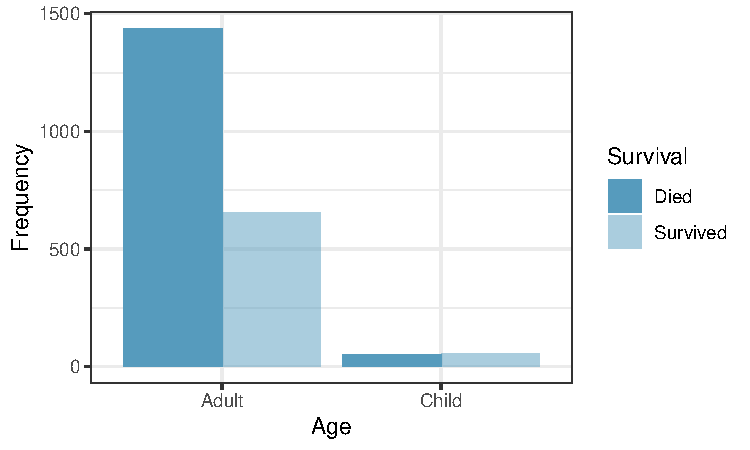
\includegraphics[width=0.5\textwidth]{2-2_categorical_data/figures/titanic_age_survival/titanic_seg_bar_dodge} \\
%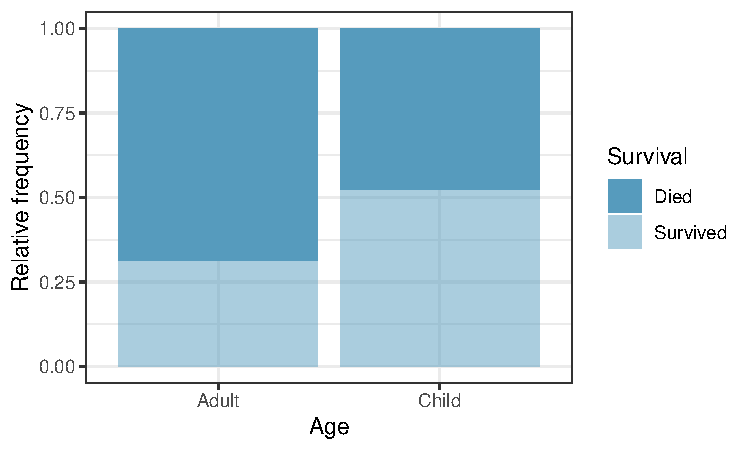
\includegraphics[width=0.5\textwidth]{2-2_categorical_data/figures/titanic_age_survival/titanic_rel_seg_bar}
\end{center}

\end{frame}

%%%%%%%%%%%%%%%%%%%%%%%%%%%%%%%%%%%%

\subsection{Mosaic plots}

%%%%%%%%%%%%%%%%%%%%%%%%%%%%%%%%%%%%

\begin{frame}
\frametitle{Mosaic plots}

\dq{What is the difference between the two visualizations shown below?}

\begin{center}
%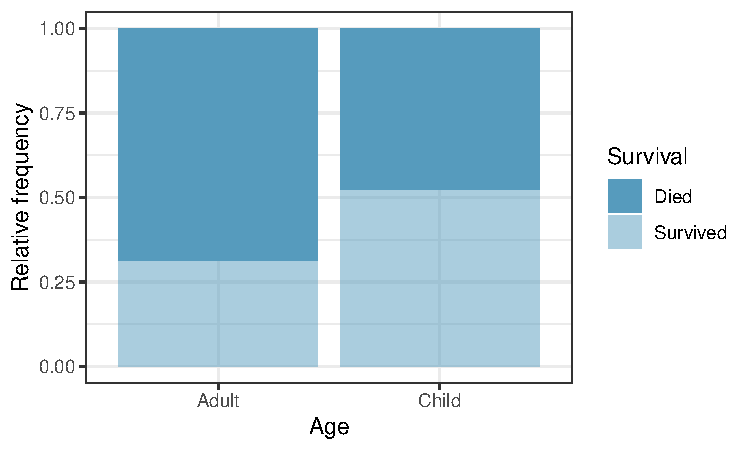
\includegraphics[width=0.5\textwidth]{2-2_categorical_data/figures/titanic_age_survival/titanic_rel_seg_bar}
%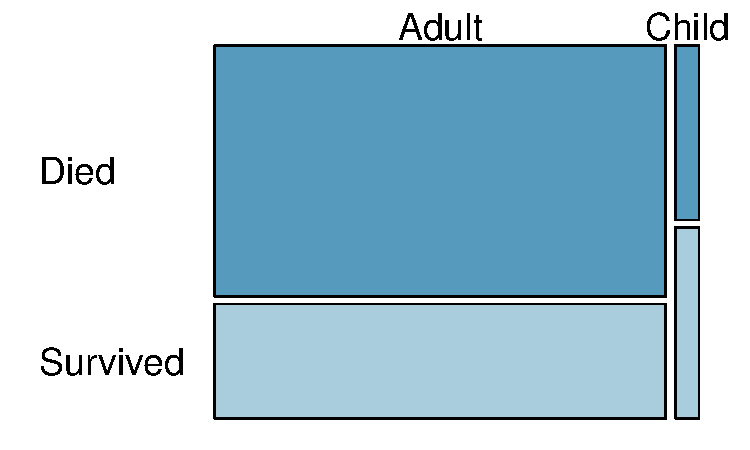
\includegraphics[width=0.5\textwidth]{2-2_categorical_data/figures/titanic_age_survival/titanic_mosaic}
\end{center}

\end{frame}

%%%%%%%%%%%%%%%%%%%%%%%%%%%%%%%%%%%%

\subsection{Pie charts}

%%%%%%%%%%%%%%%%%%%%%%%%%%%%%%%%%%%%

\begin{frame}
\frametitle{Pie charts}

\dq{Can you tell which order encompasses the lowest percentage of mammal species?}

\vspace{-0.5cm}

\begin{center}
%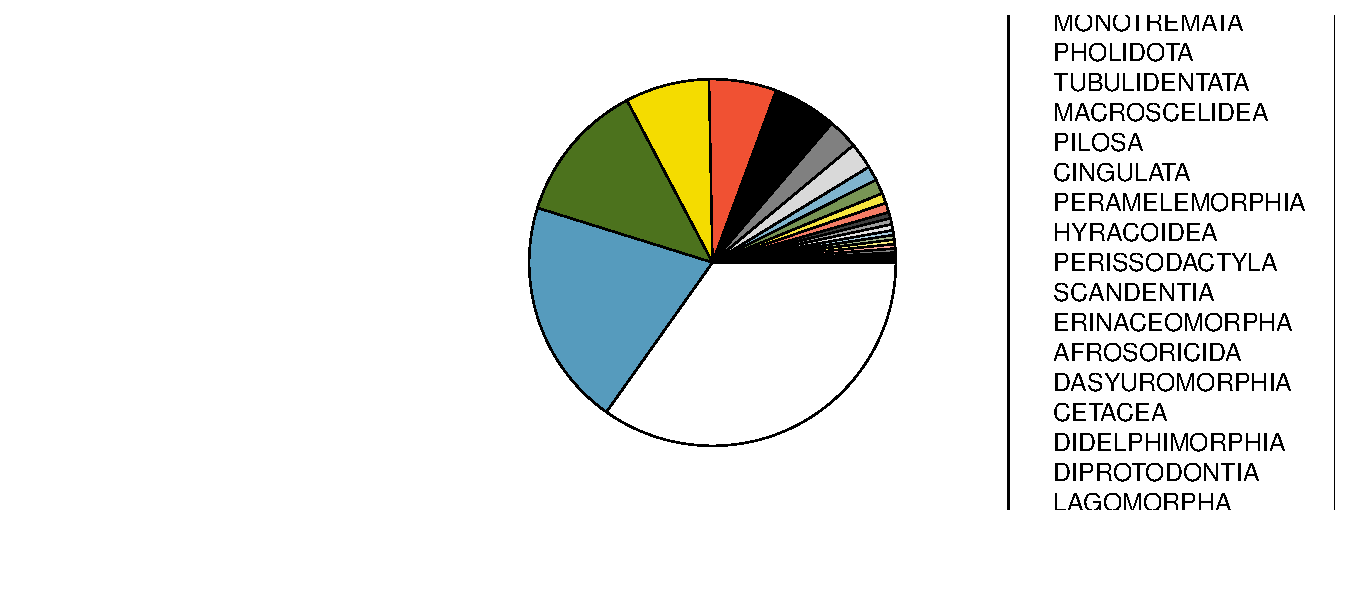
\includegraphics[width=0.4\textwidth]{2-2_categorical_data/figures/mammal_pie_chart/mammal_pie_chart}
%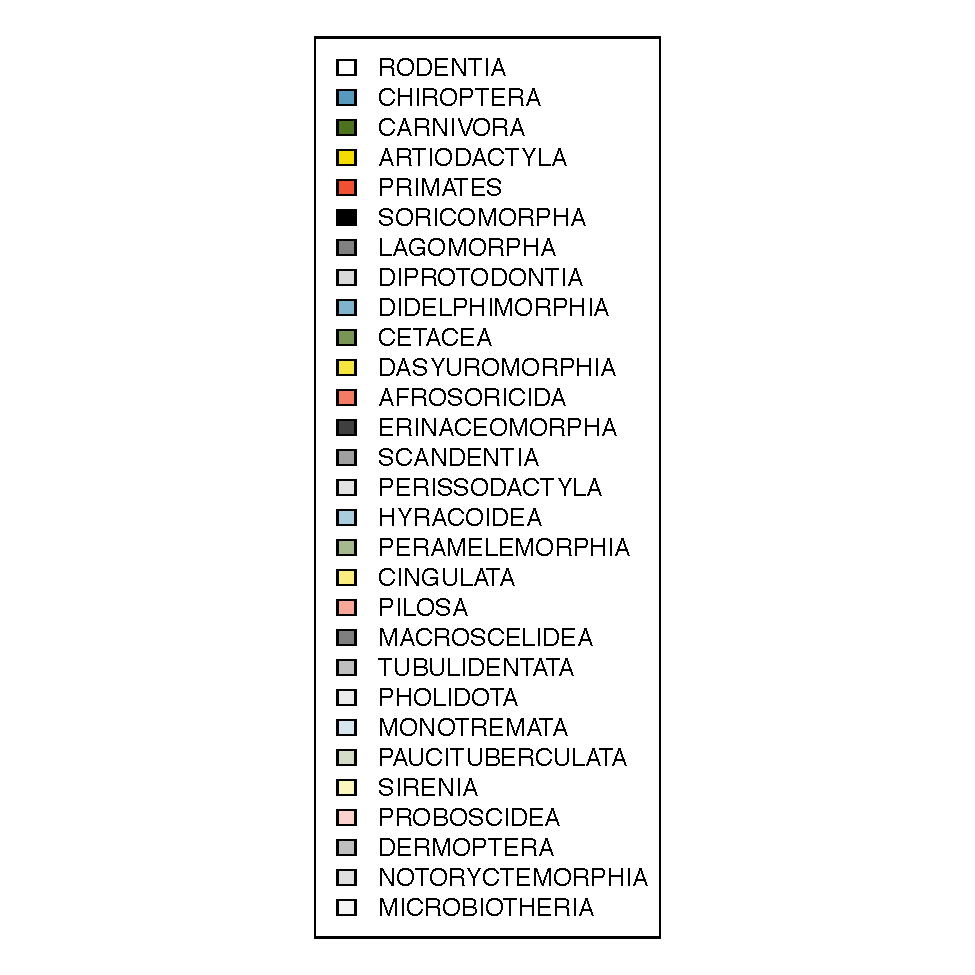
\includegraphics[width=0.2\textwidth]{2-2_categorical_data/figures/mammal_pie_chart/mammal_pie_chart_legend}
\end{center}

\ct{Data from \webURL{http://www.bucknell.edu/msw3}.}

\end{frame}


%%%%%%%%%%%%%%%%%%%%%%%%%%%%%%%%%%%%

\subsection{Comparing numerical data across groups}

%%%%%%%%%%%%%%%%%%%%%%%%%%%%%%%%%%%%

\begin{frame}
\frametitle{Side-by-side box plots}

\dq{Does there appear to be a relationship between class year and number of clubs students are in?}

\begin{center}
%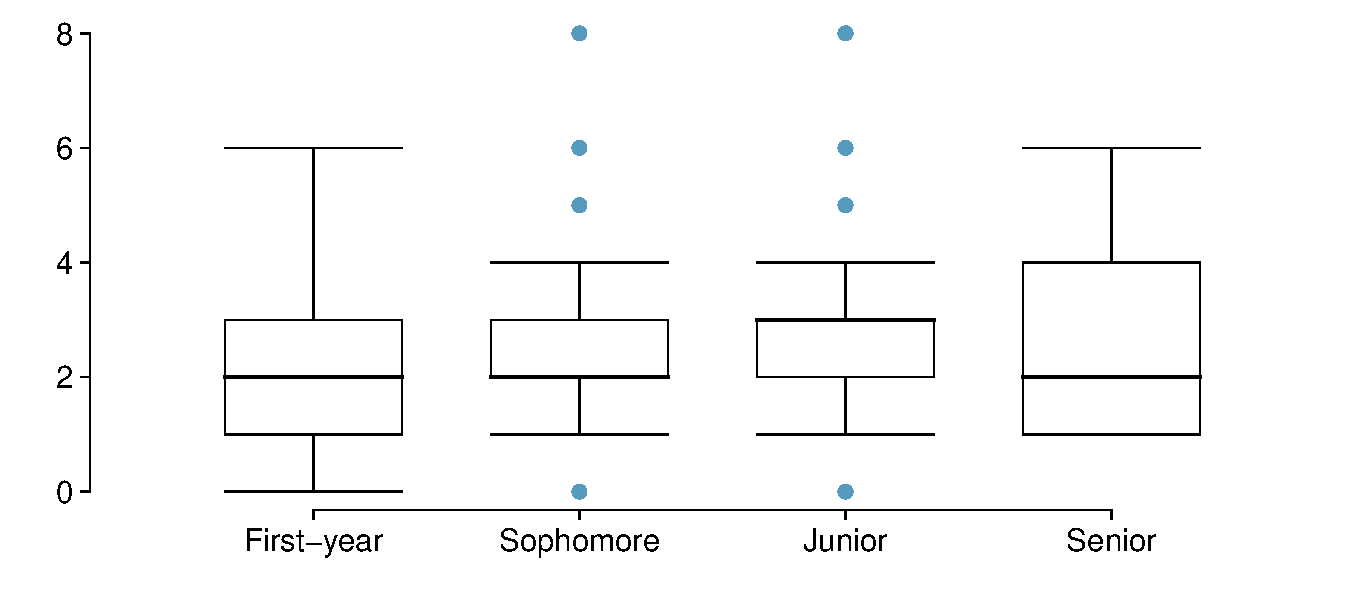
\includegraphics[width=\textwidth]{2-2_categorical_data/figures/year_clubs/year_clubs}
\end{center}

\end{frame}

%%%%%%%%%%%%%%%%%%%%%%%%%%%%%%%%%%%%

%%%%%%%%%%%%%%%%%%%%%%%%%%%%%%%%%%%%

\section{Case study: Gender discrimination}

%%%%%%%%%%%%%%%%%%%%%%%%%%%%%%%%%%%%

\subsection{Study description and data}

%%%%%%%%%%%%%%%%%%%%%%%%%%%%%%%%%%%%

\begin{frame}
\frametitle{Gender discrimination}

\begin{itemize}

\item In 1972, as a part of a study on gender discrimination, 48 male bank supervisors were each given the same personnel file and asked to judge whether the person should be promoted to a branch manager job that was described as ``routine". 

\item The files were identical except that half of the supervisors had files showing the person was male while the other half had files showing the person was female.

\item It was randomly determined which supervisors got ``male" applications and which got ``female" applications.  

\item Of the 48 files reviewed, 35 were promoted. 

\item The study is testing whether females are unfairly discriminated against.  
\end{itemize}

\dq{Is this an observational study or an experiment?} \soln{\onslide<2->{Experiment}}

\ct{B.Rosen and T. Jerdee (1974), ``Influence of sex role stereotypes on personnel decisions", J.Applied Psychology, 59:9-14.}

\end{frame}


%%%%%%%%%%%%%%%%%%%%%%%%%%%%%%%%%%%%

\begin{frame}
\frametitle{Data}

\dq{At a first glance, does there appear to be a relatonship between promotion and gender?}

\begin{center}
\begin{tabular}{ll  cc c} 
  		&				& \multicolumn{2}{c}{\textit{Promotion}} \\
\cline{3-4}
							&			& Promoted	& Not Promoted 	& Total	\\
\cline{2-5}
\multirow{2}{*}{\textit{Gender	}}	&Male 		& 21	 	& 3		& 24 	\\
							&Female		& 14	 	& 10 	 	& 24 \\
\cline{2-5}
							&Total		& 35		& 13		& 48 \\
\end{tabular}
\end{center}

\pause

\textbf{\% of males promoted: $21 / 24 = 0.875$} \\
\textbf{\% of females promoted: $14 / 24 = 0.583$}

\end{frame}

%%%%%%%%%%%%%%%%%%%%%%%%%%%%%%%%%%%%

\begin{frame}
\frametitle{Practice}

\pq{We saw a difference of almost 30\% (29.2\% to be exact) between the proportion of male and female files that are promoted. Based on this information, which of the below is true?}

\begin{enumerate}[(a)]

\item If we were to repeat the experiment we will definitely see that more female files get promoted. This was a fluke.

\item Promotion is dependent on gender, males are more likely to be promoted, and hence there is gender discrimination against women in promotion decisions. \soln{\only<2>{\red{Maybe}}}

\item The difference in the proportions of promoted male and female files is due to chance, this is not evidence of gender discrimination against women in promotion decisions. \soln{\only<2>{\red{Maybe}}}

\item Women are less qualified than men, and this is why fewer females get promoted.

\end{enumerate}

\end{frame}

%%%%%%%%%%%%%%%%%%%%%%%%%%%%%%%%%%%%

\subsection{Competing claims}

%%%%%%%%%%%%%%%%%%%%%%%%%%%%%%%%%%%%%

\begin{frame}
\frametitle{Two competing claims}

\begin{enumerate}

\item ``There is nothing going on." \\
Promotion and gender are \hl{independent}, no gender discrimination, observed difference in proportions is simply due to chance. $\rightarrow$ \hl{Null hypothesis}

\pause

\item ``There is something going on." \\
Promotion and gender are \hl{dependent}, there is gender discrimination, observed difference in proportions is not due to chance. $\rightarrow$ \hl{Alternative hypothesis}

\end{enumerate}

\end{frame}

%%%%%%%%%%%%%%%%%%%%%%%%%%%%%%%%%%%%

\begin{frame}
\frametitle{A trial as a hypothesis test}

\twocol{0.5}{0.5}
{
\begin{itemize}

\item Hypothesis testing is very much like a court trial.

\item $H_0$: Defendant is innocent \\
$H_A$: Defendant is guilty

\item We then present the evidence - collect data.

\end{itemize}
}
{
%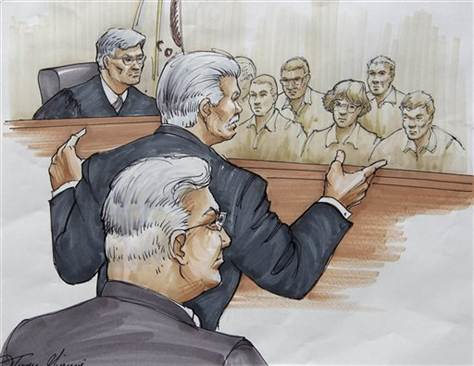
\includegraphics[width=\textwidth]{2-3_gender_discrimination/figures/trial}
}

\begin{itemize}

\item Then we judge the evidence - ``Could these data plausibly have happened by chance if the null hypothesis were true?"
\begin{itemize}
\item If they were very unlikely to have occurred, then the evidence raises more than a reasonable doubt in our minds about the null hypothesis.
\end{itemize}

\item Ultimately we must make a decision. How unlikely is unlikely?

\end{itemize}

\ct{Image from \webURL{http://www.nwherald.com/_internal/cimg!0/oo1il4sf8zzaqbboq25oevvbg99wpot}.}

\end{frame}

%%%%%%%%%%%%%%%%%%%%%%%%%%%%%%%%%%%%%

\begin{frame}
\frametitle{A trial as a hypothesis test (cont.)}

\begin{itemize}

\item If the evidence is not strong enough to reject the assumption of innocence, the jury returns with a verdict of ``not guilty".
\begin{itemize}
\item The jury does not say that the defendant is innocent, just that there is not enough evidence to convict.
\item The defendant may, in fact, be innocent, but the jury has no way of being sure.
\end{itemize}

\item Said statistically, we fail to reject the null hypothesis.
\begin{itemize}
\item We never declare the null hypothesis to be true, because we simply do not know whether it's true or not.
\item Therefore we never ``accept the null hypothesis".
\end{itemize}

\end{itemize}

\end{frame}

%%%%%%%%%%%%%%%%%%%%%%%%%%%%%%%%%%%%%

\begin{frame}
\frametitle{A trial as a hypothesis test (cont.)}

\begin{itemize}

\item In a trial, the burden of proof is on the prosecution.

\item In a hypothesis test, the burden of proof is on the unusual claim.

\item The null hypothesis is the ordinary state of affairs (the status quo), so it's the alternative hypothesis that we consider unusual and for which we must gather evidence.

\end{itemize}

\end{frame}

%%%%%%%%%%%%%%%%%%%%%%%%%%%%%%%%%%%%%

\begin{frame}
\frametitle{Recap: hypothesis testing framework}

\begin{itemize}
\item We start with a \hl{null hypothesis ($H_0$)} that represents the status quo.
\item We also have an \hl{alternative hypothesis ($H_A$)} that represents our research question, i.e. what we're testing for.
\item We conduct a hypothesis test under the assumption that the null hypothesis is true, either via simulation (today) or theoretical methods (later in the course).
\item If the test results suggest that the data do not provide convincing evidence for the alternative hypothesis, we stick with the null hypothesis. If they do, then we reject the null hypothesis in favor of the alternative.
\end{itemize}

\end{frame}

%%%%%%%%%%%%%%%%%%%%%%%%%%%%%%%%%%%%

\subsection{Testing via simulation}

%%%%%%%%%%%%%%%%%%%%%%%%%%%%%%%%%%%%%

\begin{frame}
\frametitle{Simulating the experiment...}

... under the assumption of independence, i.e. leave things up to chance. \\

\vspace{0.5cm}

If results from the simulations based on the \hl{chance model} look like the data, then we can determine that the difference between the proportions of promoted files between males and females was simply \hl{due to chance} (promotion and gender are independent). \\

\vspace{0.5cm}

If the results from the simulations based on the chance model do not look like the data, then we can determine that the difference between the proportions of promoted files between males and females was not due to chance, but \hl{due to an actual effect of gender} (promotion and gender are dependent).

\end{frame}

%%%%%%%%%%%%%%%%%%%%%%%%%%%%%%%%%%%%

\begin{frame}
\frametitle{Application activity: simulating the experiment}

\app{
Use a deck of playing cards to simulate this experiment.

\begin{enumerate}
\item Let a face card represent \textit{not promoted} and a non-face card represent a \textit{promoted}. Consider aces as face cards.
\begin{itemize}
\item Set aside the jokers.
\item Take out 3 aces $\rightarrow$ there are exactly 13 face cards left in the deck (face cards: A, K, Q, J).
\item Take out a number card $\rightarrow$ there are exactly 35 number (non-face) cards left in the deck (number cards: 2-10).
\end{itemize}
\item Shuffle the cards and deal them intro two groups of size 24, representing males and females. 
\item Count and record how many files in each group are promoted (number cards).

\item Calculate the proportion of promoted files in each group and take the difference (male - female), and record this value.

\item Repeat steps 2 - 4 many times.

\end{enumerate}
}

\end{frame}

%%%%%%%%%%%%%%%%%%%%%%%%%%%%%%%%%%%%

\begin{frame}
\frametitle{Step 1}

\begin{center}
%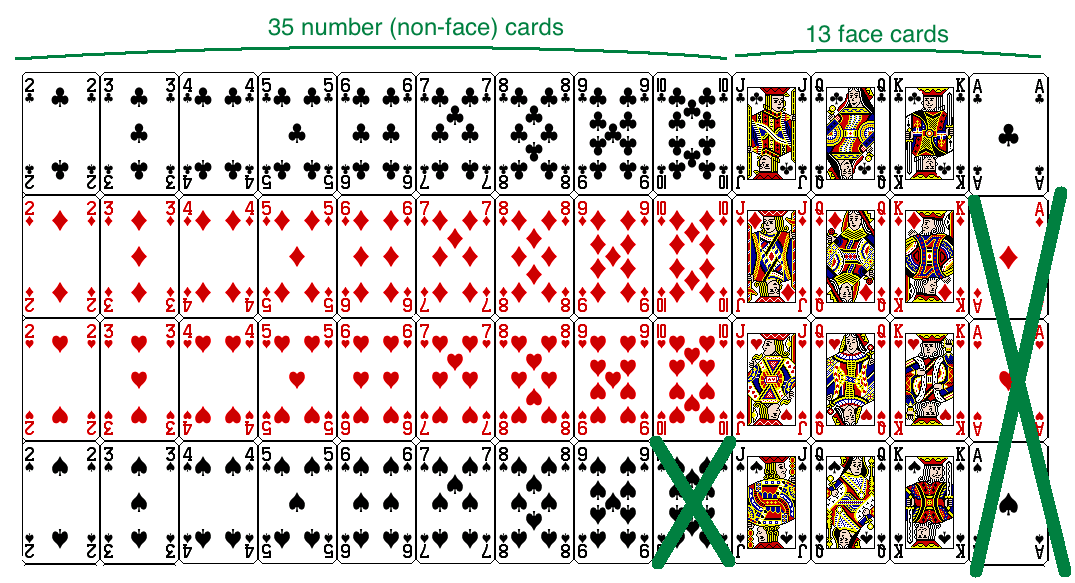
\includegraphics[width=\textwidth]{2-3_gender_discrimination/figures/step1}
\end{center}

\end{frame}


%%%%%%%%%%%%%%%%%%%%%%%%%%%%%%%%%%%%

\begin{frame}
\frametitle{Step 2 - 4}

\begin{center}
%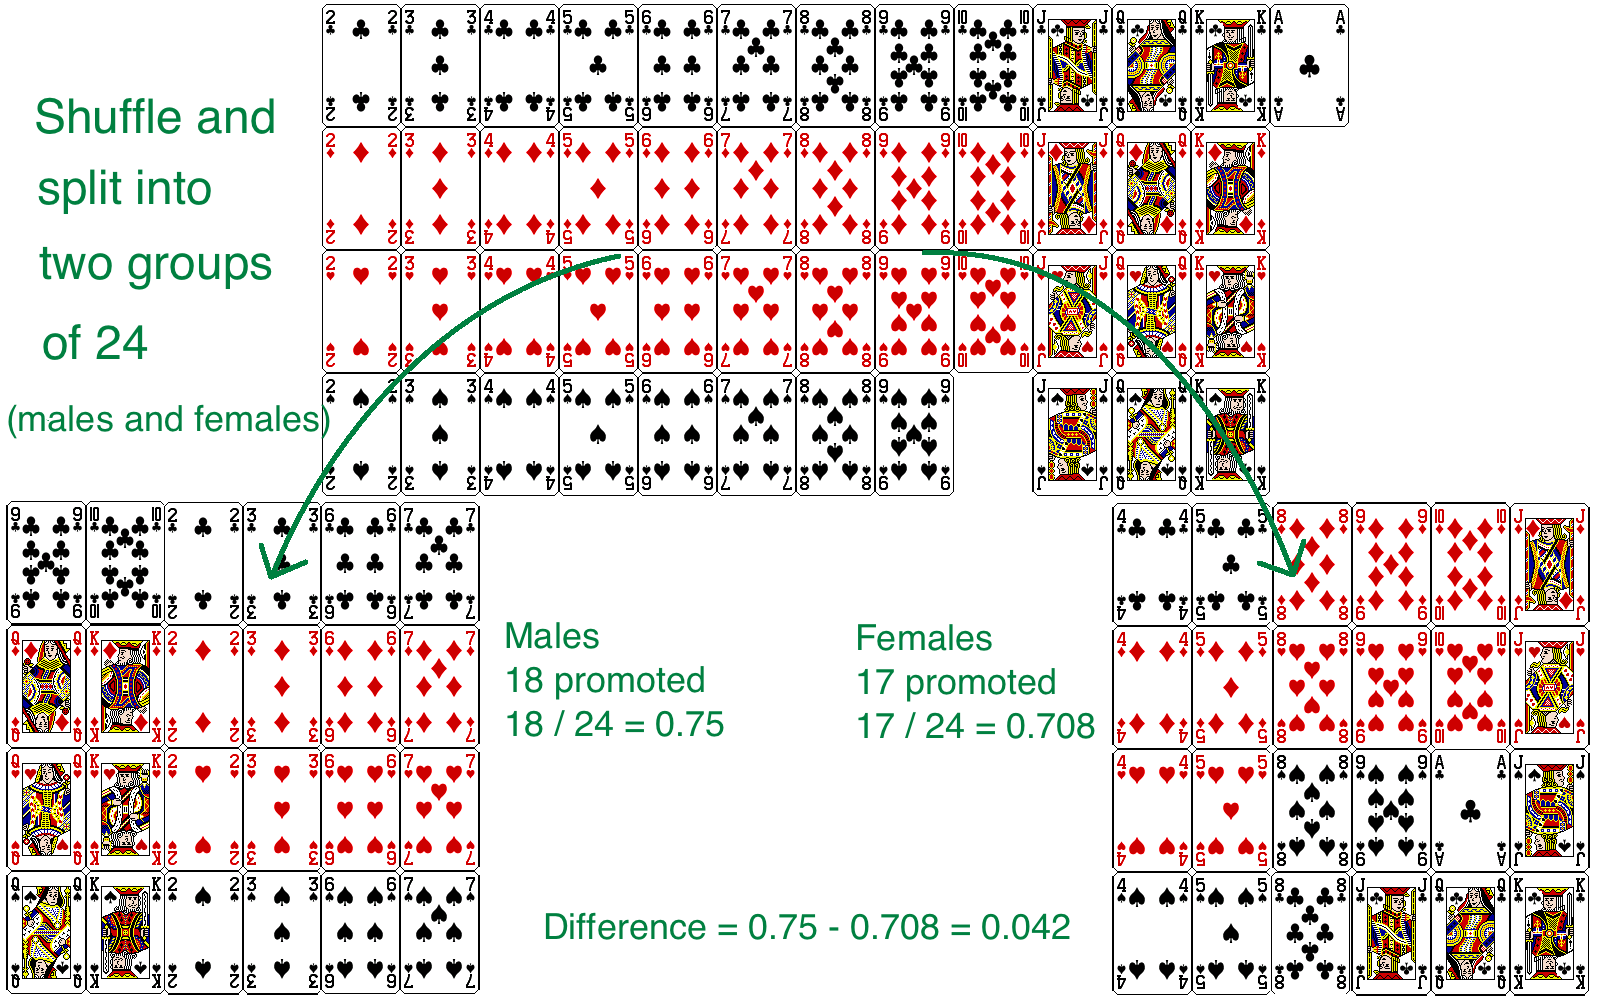
\includegraphics[width=\textwidth]{2-3_gender_discrimination/figures/step2}
\end{center}

\end{frame}


%%%%%%%%%%%%%%%%%%%%%%%%%%%%%%%%%%%%

\subsection{Checking for independence}

%%%%%%%%%%%%%%%%%%%%%%%%%%%%%%%%%%%%

\begin{frame}
\frametitle{Practice}

\pq{Do the results of the simulation you just ran provide convincing evidence of gender discrimination against women, i.e. dependence between gender and promotion decisions?}

\begin{enumerate}[(a)]
\item No, the data do not provide convincing evidence for the alternative hypothesis, therefore we can't reject the null hypothesis of independence between gender and promotion decisions. The observed difference between the two proportions was due to chance.
\solnMult{Yes, the data provide convincing evidence for the alternative hypothesis of gender discrimination against women in promotion decisions. The observed difference between the two proportions was due to a real effect of gender.}
\end{enumerate}

\end{frame}

%%%%%%%%%%%%%%%%%%%%%%%%%%%%%%%%%%%%

\begin{frame}
\frametitle{Simulations using software}

These simulations are tedious and slow to run using the method described earlier. In reality, we use software to generate the simulations. The dot plot below shows the distribution of simulated differences in promotion rates based on 100 simulations.

\begin{center}
%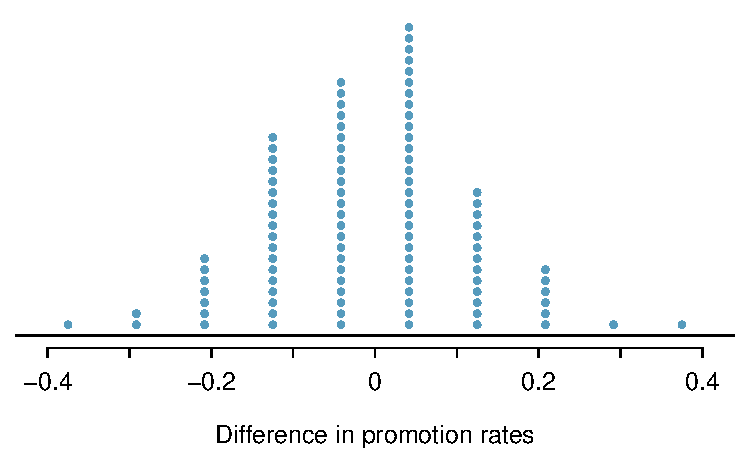
\includegraphics[width=0.8\textwidth]{2-3_gender_discrimination/figures/discRandDotPlot/discRandDotPlot}
\end{center}

\end{frame}

%%%%%%%%%%%%%%%%%%%%%%%%%%%%%%%%%%%%%

%%%%%%%%%%%%%%%%%%%%%%%%%%%%%%%%%%%%
% End document
%%%%%%%%%%%%%%%%%%%%%%%%%%%%%%%%%%%%

\end{document}